%%%%%%%%%%%%%%%%%%%%%%%%%%%%%%%%%%%%%%%%%%%%%%%%%%%%%%%%%%%%
%%% LIVECOMS ARTICLE TEMPLATE FOR BEST PRACTICES GUIDE
%%% ADAPTED FROM ELIFE ARTICLE TEMPLATE (8/10/2017)
%%%%%%%%%%%%%%%%%%%%%%%%%%%%%%%%%%%%%%%%%%%%%%%%%%%%%%%%%%%%
%%% PREAMBLE
\documentclass[9pt,tutorial]{livecoms}
% Use the 'onehalfspacing' option for 1.5 line spacing
% Use the 'doublespacing' option for 2.0 line spacing
% Use the 'lineno' option for adding line numbers.
% Use the "ASAPversion' option following article acceptance to add the DOI and relevant dates to the document footer.
% Use the 'pubversion' option for adding the citation and publication information to the document footer, when the LiveCoMS issue is finalized.
% The 'bestpractices' option for indicates that this is a best practices guide.
% Omit the bestpractices option to remove the marking as a LiveCoMS paper.
% Please note that these options may affect formatting.

\usepackage{lipsum} % Required to insert dummy text
\usepackage[version=4]{mhchem}
\usepackage{siunitx}
\DeclareSIUnit\Molar{M}
\usepackage[italic]{mathastext}
\graphicspath{{figures/}}

%%%%%%%%%%%%%%%%%%%%%%%%%%%%%%%%%%%%%%%%%%%%%%%%%%%%%%%%%%%%
%%% IMPORTANT USER CONFIGURATION
%%%%%%%%%%%%%%%%%%%%%%%%%%%%%%%%%%%%%%%%%%%%%%%%%%%%%%%%%%%%

\newcommand{\versionnumber}{0.2}  % you should update the minor version number in preprints and major version number of submissions.
\newcommand{\githubrepository}{\url{https://github.com/TMB-CSB/hdxer_tutorials_livecoms}}

%%%%%%%%%%%%%%%%%%%%%%%%%%%%%%%%%%%%%%%%%%%%%%%%%%%%%%%%%%%%
%%% ARTICLE SETUP
%%%%%%%%%%%%%%%%%%%%%%%%%%%%%%%%%%%%%%%%%%%%%%%%%%%%%%%%%%%%
\title{Combining hydrogen-deuterium exchange experiments with molecular simulations: Tutorials and applications of the HDXer ensemble reweighting software [Article v\versionnumber]}

\author[1]{Paul Suhwan Lee}
\author[1*\authfn{1}]{Richard T. Bradshaw}
\author[2]{Fabrizio Marinelli}
\author[3]{Kyle Kihn}
\author[3]{Ally Smith}
\author[3]{Patrick L. Wintrode}
\author[3]{Daniel J. Deredge}
\author[2]{José D. Faraldo-Gómez}
\author[1*]{Lucy R. Forrest}
\affil[1]{Computational Structural Biology Section, National Institute of Neurological Disorders and Stroke, National Institutes of Health, Bethesda, MD, USA}
\affil[2]{Theoretical Molecular Biophysics Section, National Heart, Lung, and Blood Institute, National Institutes of Health, Bethesda, MD, USA}
\affil[3]{Department of Pharmaceutical Sciences, School of Pharmacy, University of Maryland, Baltimore, MD, USA}

\corr{richard.bradshaw@kcl.ac.uk}{RTB}  % Correspondence emails.  
\corr{lucy.forrest@nih.gov}{LRF}

\orcid{Paul Suhwan Lee}{0000-0003-2658-4641}
\orcid{Richard T. Bradshaw}{0000-0002-8652-4301}
\orcid{Fabrizio Marinelli}{0000-0003-0044-6718}
\orcid{Kyle Kihn}{0000-0002-0502-1332}
\orcid{Ally Smith}{0000-0003-4539-1714}
\orcid{Patrick L. Wintrode}{0000-0003-1866-9397}
\orcid{Daniel J. Deredge}{0000-0002-6897-6523}
\orcid{José D. Faraldo-Gómez}{0000-0001-7224-7676}
\orcid{Lucy R. Forrest}{0000-0003-1855-7985}

\presentadd[\authfn{1}]{Department of Chemistry, King's College London, Britannia House, 7 Trinity Street, London SE1 1DB, UK}

\blurb{This LiveCoMS document is maintained online on GitHub at \githubrepository; to provide feedback, suggestions, or help improve it, please visit the GitHub repository and participate via the issue tracker.}

%%%%%%%%%%%%%%%%%%%%%%%%%%%%%%%%%%%%%%%%%%%%%%%%%%%%%%%%%%%%
%%% PUBLICATION INFORMATION
%%% Fill out these parameters when available
%%% These are used when the "pubversion" option is invoked
%%%%%%%%%%%%%%%%%%%%%%%%%%%%%%%%%%%%%%%%%%%%%%%%%%%%%%%%%%%%
\pubDOI{10.XXXX/YYYYYYY}
\pubvolume{<volume>}
\pubissue{<issue>}
\pubyear{<year>}
\articlenum{<number>}
\datereceived{Day Month Year}
\dateaccepted{Day Month Year}

%%%%%%%%%%%%%%%%%%%%%%%%%%%%%%%%%%%%%%%%%%%%%%%%%%%%%%%%%%%%
%%% ARTICLE START
%%%%%%%%%%%%%%%%%%%%%%%%%%%%%%%%%%%%%%%%%%%%%%%%%%%%%%%%%%%%

\begin{document}

\begin{frontmatter}
\maketitle

\begin{abstract}
Hydrogen-deuterium exchange (HDX) in proteins is a subtle yet detailed reporter of protein structure and dynamics, and, coupled to mass spectrometry, has become a powerful structural biology tool for probing an increasingly large array of protein systems.
Computer simulations are often used to help rationalize experimental observations of exchange, but interpretations have frequently been limited to simple, subjective, correlations between microscopic dynamical fluctuations and the observed macroscopic exchange behavior.
With this in mind, the HDX ensemble reweighting approach and associated software, HDXer, has been designed to aid the objective interpretation of HDX data using molecular simulations.
HDXer has two main functions; first, to predict H-D exchange rates from a candidate ensemble of protein structures, for example from molecular simulations, and second, to objectively reweight the conformational populations present in a candidate ensemble to conform to experimental exchange data.
In this article, we first describe the HDXer approach, theory, and implementation. 
We then guide users through a suite of tutorials, demonstrating practical applications of experimental data preparation, predicting HDX levels from molecular simulations, and performing ensemble reweighting analyses.
Finally, we provide a practical discussion of the capabilities and limitations of the HDXer methods, including recommendations for a user's own analyses.
Overall, this article is intended to provide an up-to-date, pedagogical counterpart to the software, which is freely available at \url{https://github.com/TMB-CSB/HDXer}.
\end{abstract}

\end{frontmatter}


\section{Introduction}
A pioneering descriptive framework, developed by Linderstrøm-Lang and co-workers, first linked the hydrogen exchange rates of backbone amide functional groups directly to protein structure in the 1950s \cite{Hvidt1954, Englander1997}. 
This concept provided the foundation for the subsequent development of hydrogen-deuterium exchange (HDX) measurements as a sensitive, label-free probe of protein conformation and dynamics in solution, and due to these advances HDX is now a valuable addition to the modern structural biology toolbox. 
In recent years, successful applications of HDX measurements have proliferated, in part due to advancements in technologies used to perform, analyze, and process HDX experiments. 
In particular, experiments that couple HDX to mass spectrometry measurements of the deuterium uptake (HDX-MS) have become the most widespread for applications of HDX to the dynamics of proteins in solution.
HDX-MS offers particular advantages over NMR-based exchange measurements for many applications, such as the determination of exchange data for large protein systems or complexes and with low sample amounts \cite{Oganesyan2018, Engen2020, James2021}.

Within the protein environment, the canonical mechanisms for backbone amide deuterium exchange require the amide hydrogen to be exposed and accessible, at least transiently, to a nearby catalytic solvent molecule, OD$^-$, or D$_3$O$^+$ ion \cite{Hvidt1966, Englander1983}.
For a folded protein, therefore, the rate of exchange reports on the extent to which local protein flexibility, conformational changes, or global unfolding, expose the amide to nearby catalysts, and result in deuterium exchange \cite{Hvidt1966, Englander1997, Englander1983, Oganesyan2018}.
The connection between deuterium exchange and structural flexibility offers the possibility to interpret HDX in a structural context.
To do so, the measured local exchange rates, whether at individual residue resolution or averaged over oligopeptide fragments as in the case of HDX-MS data, are typically correlated with specific structural features. 
These features include secondary structure, H bonding, or accessibility to solvent and can be extracted from either experimentally-determined or modeled structures of the protein of interest.

A clear limitation of using single structures to interpret HDX data, however, is that this approach underutilizes the information inherently encoded in the experimental measurement.
Specifically, HDX measurements, in theory, contain information describing the complete structural ensemble as well as the equilibrium conformational dynamics of the protein under investigation.
An important requirement for the next generation of HDX studies will therefore be the ability to rigorously decode the dynamical information present in the observed data, to enable high-resolution, quantitative, robust, and objective structural ensembles to be derived directly from the experimental measurements.
With this in mind, we developed the HDX ensemble reweighting (HDXer) approach \cite{Bradshaw2020}, and associated software, to facilitate quantitative and objective structural interpretation of HDX-MS data.

The HDXer software has two main functions:

\begin{enumerate}
\item To predict the average structural protection afforded to each backbone amide, \textit{i}, in a protein structural ensemble (the Protection Factor, \textit{P\textsubscript{i}}), for a given empirical predictive model. These values can then be translated into an overall H-D exchange rate and fractional deuteration, for any combination of residues in a peptide segment, at any given timepoint, thereby allowing direct comparison to experimental HDX-MS data;

\item To optimally fit an initial protein structural ensemble to a target set of HDX-MS data, taking into account all potential sources of uncertainty, using a maximum entropy reweighting procedure \cite{Pitera2012, Boomsma2014, Marinelli2019}. This approach adjusts the populations of each conformation in the ensemble such that the overall average structural protection of each backbone amide conforms ideally to the experimental data.
\end{enumerate}

We recognize that these techniques may be unfamiliar even to colleagues with experience in HDX and/or computer simulations. 
Therefore, to increase the accessibility of HDXer to the wider community, we present here a suite of tutorials, available as interactive Jupyter notebooks, that describe how users can prepare, perform, and interpret HDXer analyses. 
We also provide a practical discussion of key aspects of the theoretical underpinnings of the HDXer approach, as well as suggestions for how users can validate the reliability and robustness of their applications of HDXer.
After completing the tutorials, which are available alongside the HDXer software itself in the GitHub repository (\url{https://github.com/TMB-CSB/HDXer}), and reading the accompanying discussion provided here, users should be able to:

\begin{itemize}
\item prepare and format raw experimental HDX-MS data, such as that created by commonly-used MS analysis packages, ready for analysis with HDXer;
\item compute predicted per-residue Protection Factor values and deuterated fractions for peptide segments from an ensemble of candidate structures (obtained, for example, from molecular dynamics (MD) simulations);
\item reweight a candidate structural ensemble so that its predicted HDX levels fit those in a target set of experimental HDX-MS data;
\item analyze a reweighted ensemble to assess both the level of agreement with the target data and the bias that was applied to adjust the populations of individual conformations in the ensemble;
\item structurally characterize a reweighted ensemble;
\item understand the potential sources of uncertainty in HDXer analyses, how that uncertainty can impact the accuracy of structural interpretations, and, relatedly, how to apply approaches to investigate and address inaccuracies in the user's specific applications.
\end{itemize}

The tutorials are self-contained and therefore require no additional data or resources beyond those detailed in the 'Prerequisites' sections below. 
In terms of background knowledge, we provide a general introduction to the theoretical concepts of both HDX and ensemble reweighting in section \ref{interpretingexptdata_sect}, which also contains suggestions for sources of more detailed information for the interested user.

\subsection{Tutorial prerequisites}
\subsubsection{Background knowledge}
Our explanations of the HDXer method and tutorials assume that users are familiar with common ideas and terminology of physical chemistry, thermodynamics, and statistical ensembles of molecules.
Beyond these concepts our article aims to provide users with a self-contained solid foundation in the specific theory underpinning ensemble reweighting and computational HDX predictions, primarily within section \ref{interpretingexptdata_sect}.
In addition, however, users should have a good understanding of the two input data sources for HDXer analyses, namely structural ensembles generated \textit{via} molecular modeling and simulation, and the experimental measurement of protein HDX-MS data.

In practical terms, users should be familiar with the process of preparing and performing simulations, or generating models, with their chosen software. 
This process includes carefully selecting the initial seed or template structure (e.g. determined by X-ray crystallography), modelling unresolved residues to match the sequence of the experimental protein construct, choosing protonation states of ionizable residues, incorporating any required ligands and describing them with reliable parameters, and appropriately representing the protein environment (e.g. oligomerization, complexation, or membrane embedding of the protein).
Obtaining a relevant, fully-representative candidate structural ensemble is crucial for accurate HDXer analyses.
The decision as to whether the ensemble should be broadened, or narrowed, can be informed by post-reweighting checks, as described in section \ref{robustness_sect}.

In terms of computational background, to benefit from the tutorials users will need a basic level of familiarity with Unix environments and the command line interface (e.g., making and moving files and directories).
A basic knowledge of Python is also desirable for users wishing to move beyond the Juptyer notebooks and apply HDXer to their own systems. 

Finally, users should be familiar with their target experimental HDX data, including the conditions under which it was obtained, the level of deuterium back-exchange (for HDX-MS data), and the proposed kinetic mechanism of exchange for each amide or peptide.
HDXer analyses assume that the target exchange data has been normalized for back exchange and for the total deuterium ratio in the solution (e.g., by normalizing uptake to a fully-deuterated control sample), and that the data represent residues and peptides undergoing an EX2-type exchange mechanism, as explained further in section \ref{predictivemodel_sect}.

\subsubsection{Software}\label{Software_sect}
The HDXer tutorials are written in Python 3.7, and are available as Jupyter notebooks, downloadable from the HDXer GitHub repository at \url{https://github.com/TMB-CSB/HDXer}.
Users should use the git version control software to clone and update the HDXer package. Installation instructions are documented in the \texttt{README} file within the repository.
We recommend creating a separate Python virtual environment for HDXer analyses, which has the following dependencies: MDTraj ($\geqslant$1.9.3) \cite{McGibbon2015MDTraj}, NumPy ($\geqslant$1.18.1) \cite{Harris2020}, Matplotlib ($\geqslant$3.2.0) \cite{Hunter:2007}, Pytest ($\geqslant$5.3.5) \cite{pytest5.3}, and Jupyterlab ($\geqslant$3.0) \cite{project_jupyter}.
To recreate the testing environment for HDXer, a Conda environment file, \texttt{HDXER\_ENV.yml}, is available in the HDXer GitHub repository.
The tutorials have the same dependencies as the software itself, and thus if the HDXer package has been successfully installed, no additional software is required.

\subsubsection{Hardware}
The HDXer tutorials have modest hardware requirements and are designed to work with any, relatively modern, consumer desktop or laptop.
Individual HDXer analyses use only a single CPU thread, though time and memory requirements depend on the size of the candidate structural ensemble, and on the number of datapoints being targeted during reweighting.
If the underlying NumPy installation has been installed with support for multi-threading, analyses may experience a performance boost for the matrix operations.
However, such an improvement is not guaranteed, so we recommend users run their own tests if they wish to take advantage of multi-threading.

\subsection{Interpreting experimental data with ensemble reweighting techniques}\label{interpretingexptdata_sect}

HDXer contributes to a growing toolbox of computational strategies that have been developed to integrate experimental data directly into the computational modeling and simulation process \cite{Bonomi2017, Kofinger2019, Orioli2020}.
These methods are designed to augment low-resolution experimental structural data by selecting or refining high-resolution structural models so as to optimally describe the underlying experimental observable.
This process, frequently referred to under the umbrella term of 'ensemble refinement', complements existing high-resolution structural biology techniques, such as X-ray crystallography or cryo-electron microscopy, and can provide information on solution-state structure and dynamics \cite{Rozycki2011, Marinelli2015, Marinelli2019, Bottaro2018, Bengtsen2020, Cesari2016, Hustedt2018, Kofinger2019}.

We classify HDXer itself as a \textit{post-hoc} maximum entropy ensemble reweighting method \cite{Pitera2012, Boomsma2014}. 
Put more simply, HDXer minimally biases the relative populations of frames in a previously-generated candidate structural ensemble, such that the predicted HDX-MS data of the ensemble conform to a target (experimental) set of HDX-MS data, within a chosen level of uncertainty.
This process is illustrated in Figure \ref{fig:reweightingschematic}.
\begin{figure}
    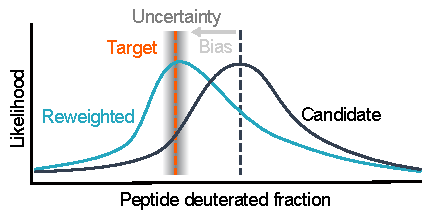
\includegraphics[width=0.98\linewidth]{Fig1_HDXer_schematic_v4.pdf}
    \caption{Schematic of HDX ensemble reweighting for a given peptide segment. The calculated HDX-MS deuterated fraction for each frame in a candidate ensemble of structures is described by an initial distribution of predicted HDX-MS data (black solid line), with an ensemble average (black dashed line) that differs from the experimentally-measured value (orange dashed line). Maximum-entropy reweighting applies the minimum possible bias (light gray arrow) to create a corrected distribution (blue line), with an ensemble average that now conforms to the experimental value within a defined level of uncertainty (dark gray shading).}
    \label{fig:reweightingschematic}
\end{figure}

Independent of the nature of the experimental data used as the target, any \textit{post-hoc} maximum entropy ensemble reweighting procedure requires three key ingredients \cite{Orioli2020}:

\begin{enumerate}
\item An initial ensemble of structures;
\item A predictive model (also known as the 'forward' model) to predict the experimental observable of interest from the coordinates of the structures in that ensemble;
\item An algorithm to fit the ensemble to the experimental data, taking into account the uncertainties in all stages of the analysis. 
\end{enumerate}
We expand upon the details and requirements of each of these three elements in the following sections.

\subsubsection{The initial structural ensemble}\label{initialensemble_sect}
As an ensemble reweighting technique, the overall goal of an HDXer analysis is to modify the relative populations (or 'weights') of frames in an initial structural ensemble.
In this context, new frames will not be added to the ensemble even if the agreement with target data is poor. 
Therefore, the initial structural ensemble should ideally, comprehensively cover all relevant protein conformational space (i.e., the 'true' conformations present in the experimental ensemble).
On the other hand, it is important to note that the relative weights of each frame can be increased or decreased, but individual frames cannot be removed from the ensemble. 
Therefore, the presence of 'irrelevant' structures (i.e. conformations not present in the experiment) should be kept to a minimum.

Atomic-resolution MD simulations initiated with a high-resolution, experimentally-determined structure, constitute a well-established approach to explore the conformational space of biomolecules in solution \cite{Huggins2019}. 
Such simulations, by definition, sample a Boltzmann distribution of states, making them a straightforward and rigorous tool for generating a candidate ensemble of structures for HDXer analyses, and as such have been used in the HDXer tutorials described here.
Nevertheless, the exhaustiveness of conformational sampling obtained using MD simulations is limited by the overall protein size, the available computational resources, and the conformational diversity of the experimentally-determined structures used to initiate simulations.
In some cases, therefore, classical (unbiased) simulations may not sufficiently sample the relevant conformational space, or may become kinetically trapped in regions of conformational space that are not representative of the dynamics observed experimentally.

To mitigate this problem, candidate ensembles can be generated using strategies for enhancing conformational sampling \cite{Allison2020}.
A straightforward approach, for example, would be to combine ensembles from multiple simulations, each initiated with a differing structure.
Such a strategy would enable the inclusion of any relevant alternative (e.g. active vs. inactive, apo vs. holo) conformational states that may not be accessed during a simulation initiated with only one of those states.
A candidate ensemble may be further extended by using so-called biased simulation methodologies, such as Accelerated MD \cite{Hamelberg2004}, Hamiltonian Replica Exchange \cite{Fukunishi2002}, or Metadynamics \cite{Laio2002}, which the user can design to sample regions of the protein conformational free energy surface that are of interest, but not well explored by other approaches.
In cases where experimental structures are unavailable, candidate ensembles may even be generated by using homology or \textit{de novo} modeling.

Generally speaking, the HDXer software will reweight a candidate ensemble of any origin.
However, the further the initial set of candidate structures is from an equilibrium Boltzmann distribution of states, the greater the level of bias that is likely required to reweight the ensemble to conform to the experimental data, because many poorly-conforming structures will need to be downweighted.
When high levels of bias are applied, small changes in the input information or target data can have an exaggerated impact on the final results, making it difficult for users to characterize the robustness of the reweighted ensemble and to identify overfitting (see Section \ref{robustness_sect}).
Thus, in general, the reliability of the reweighting will be lessened if the candidate ensemble contains too much 'structural noise', for example from irrelevant conformations not representative of local free energy minima.
In summary, if users choose to generate candidate ensembles using enhanced sampling methodologies, they should endeavor to ensure that the candidate structures comprehensively represent the equilibrium dynamics of the system. 

\subsubsection{Predictive models for HDX}\label{predictivemodel_sect}
Within the Linderstrøm-Lang model for hydrogen exchange, each backbone amide can exist in either an 'open', accessible and exchange-competent state (O), or a 'closed', protected and exchange-non-competent state (C) \cite{Hvidt1966, Englander1997, Jensen2016}.
Interconversion between the O and C states is governed by individual rate constants; $k_{\textnormal{op}}$ for the opening conformational change, and $k_{\textnormal{cl}}$ for closing.
The exchange reaction itself, which is governed by an intrinsic chemical exchange rate constant $k_{\textnormal{int}}$, is only possible from the amide O state.
The relationship between these rate constants (equation \ref{LL_exch_model_eqn}) gives rise to two alternative kinetic regimes for the calculation of the experimentally-observed overall rate of exchange, $k_{\textnormal{HX}}$ (equation \ref{EX1_EX2_eqn}) \cite{Jensen2016, Ferraro2004, James2021}.

\begin{equation}\label{LL_exch_model_eqn}
\ce{(N-H)_C <=>[$k$_{op}][$k$_{cl}] (N-H)_O <=>[$k$_{int}][] (N-D)_O <=>[$k$_{cl}][$k$_{op}] (N-D)_C}
\end{equation}
\begin{equation}\label{EX1_EX2_eqn}
\begin{gathered}
\textnormal{EX1:  } k_{\textnormal{int}} >> k_{\textnormal{cl}}  ,  k_{\textnormal{HX}} = k_{\textnormal{op}} \\
\textnormal{EX2:  } k_{\textnormal{int}} << k_{\textnormal{cl}}, k_{\textnormal{HX}} =
\frac{k_{\textnormal{op}}}{k_{\textnormal{cl}}}k_{\textnormal{int}}
\end{gathered}
\end{equation}

Amides can require vastly different structural transitions to reach an exchange-competent O state \cite{Hvidt1966, Englander1983, Skinner2012mechanisms, Skinner2012models}. 
The protein backbone of some structural features may only be accessible to exchange following a local or global unfolding motion, refolding from which is likely to be far slower than the intrinsic rate of exchange.
Amides in these structures will therefore undergo exchange with EX1 kinetics, with an overall rate directly proportional to that of the unfolding conformational change, $k_\textnormal{op}$.

Amides that exhibit EX2 exchange, common under native conditions, access exchange-competent states \textit{via} smaller conformational fluctuations, in which the rate of refolding to the C state is far faster than the chemical exchange reaction.
Here, the observed HDX rate is proportional to the equilibrium of the amide O/C states, or equivalently to the 'opening' conformational free energy change $\Delta G_{\textnormal{op}}$ (equation \ref{PF_deltaG_eqn}).
The O/C equilibrium is also frequently described in the context of the amide protection factor, $P_i$, which represents the ratio $\frac{k_\textnormal{cl}}{k_\textnormal{op}}$, or can also be calculated from the experimentally-measurable ratio $\frac{k_\textnormal{int}}{k_\textnormal{HX}}$.

\begin{equation}\label{PF_deltaG_eqn}
{\Delta}G_{\textnormal{op}} = -RT\ln{\frac{k_{\textnormal{op}}}{k_{\textnormal{cl}}}} = RT\ln{P_i}
\end{equation}

Models to estimate protection factor provide an opportunity to interpret EX2 exchange in a structural context, and typically fall into two families.
The first approach requires extensive sampling of the amide C and O states, from which the C/O equilibrium constant $P_i$ is calculated directly by classifying each conformation as 'open' or 'closed', and counting the relative populations (i.e. probabilities) of each state \cite{Persson2015, Liu2012}.
A common alternative technique is to use an empirical scoring function that correlates protein structural and dynamical features, observed in an ensemble of structures, with the amide $\Delta G_\textnormal{op}$ \cite{VendruscoloPaci2003, BestVendruscolo2006, Kieseritzky2006, Ma2011, Petruk2013, Park2015, Markwick2019}.
The latter procedure requires no knowledge or definition of the O state structural constitution for each amide. 
Indeed, the parameterization of empirical $P_i$ models has often made use of structures from equilibrium MD simulations exploring dynamics on ns-µs timescales, which would predominantly sample the well-folded C state for each amide, and neglect O-state transitions that may occur on longer timescales.
Interpreting experimental H-D exchange with empirical $P_i$ models therefore characterizes the amide C state, alongside any rapid and transient O state fluctuations on short (ps-ns) timescales well-sampled by the parameterization process.
O state structures resulting from large or slow dynamic transitions are unlikely to be incorporated in the structural ensembles modeled using empirical $P_i$ predictions, which highlights the importance of correctly classifying EX1 and EX2 behavior when choosing experimental data to interpret \textit{via} predictive models.
Fortunately, a simple analysis of the peptide mass envelopes obtained in HDX-MS experiments often allows classification of individual peptides into EX1, EX2, or mixed EX1/EX2 exchangers for this purpose \cite{Jensen2016, Ferraro2004, James2021}.

Currently, HDXer applies the commonly-used phenomenological model \cite{VendruscoloPaci2003, BestVendruscolo2006}, which estimates \textit{P\textsubscript{i}} for each backbone amide as an ensemble average function of the number of heavy atom contacts, \textit{N\textsubscript{C,i}}, and H bonds, \textit{N\textsubscript{H,i}}, formed by the amide NH group:
\begin{equation}\label{pf_model}
    \ln{P_i} = \langle \beta_\textnormal{C} N_{\textnormal{C},i} + \beta_\textnormal{H} N_{\textnormal{H},i} \rangle.
\end{equation}
Consequently, in order to count the H bonds and contacts formed by each backbone amide, HDXer requires a fully atomistic representation of the protein, including hydrogen atoms.
Structural protection from other sources, such as bound ligands, co-factors, or lipid bilayers, can also be included in Equation \ref{pf_model}, if these elements are present in the candidate structural ensemble.

However, it should be noted that the phenomenological model includes two empirical scaling parameters reflecting the relative contributions of heavy atom contacts and H bonding to structural protection.
The default values for these scaling factors ($\beta_\textnormal{C} = 0.35, \beta_\textnormal{H} = 2.0$) were originally parameterized with a training dataset of globular, monomeric proteins \cite{BestVendruscolo2006}, and therefore may not be suitable for proteins that obtain substantial structural protection from non-protein sources, for example from embedding in a lipid bilayer.
HDXer can accommodate such adjustments to the predictive model as it allows $\beta_\textnormal{C}$ and $\beta_\textnormal{H}$ to be treated either as user-definable constants or as optimizable parameters during reweighting.

Using the empirically-calculated protection factors, HDXer can then calculate the fractional deuteration of each amide at a nominal deuterium exposure time, $D_{i,t}$, as:
\begin{equation}\label{Df_eqn}
    D_{i,t} = 1 - \exp\left( \frac{-k_{\textnormal{int},i}}{P_i}t \right)
\end{equation}
where the intrinsic rates of exchange for each amide, $k_{\textnormal{int},i}$, are automatically computed by HDXer based on the local sequence of each residue using experimentally-determined reference data \cite{Bai1993, Nguyen2018}. 
Since those intrinsic rates depend on conditions such as the pD and temperature of deuteration, HDXer also allows the user to adjust the latter parameters to be consistent with their particular experimental conditions.

\subsubsection{Ensemble reweighting using the maximum entropy principle}\label{maxent_theory_sect}
The theory of the maximum entropy principle and how it can be used to integrate experimental data into molecular simulations has been well described elsewhere \cite{Pitera2012, Boomsma2014, Marinelli2019, Hummer2015}, and the derivation of the method for HDX data was provided in our original HDXer publication \cite{Bradshaw2020}.
We recommend that users become comfortable with the theory of the approach by following these texts. 
Here, we provide a general overview of the concept of maximum entropy reweighting, which is required for users to understand the terminology used in the tutorials and how to interpret the results.

At its core, the HDXer process applies an energy bias to the underlying potential energy of each frame in the initial candidate ensemble, $U(X)$, to create a new, corrected, potential, $U_{\textnormal{corr}}(X)$:
\begin{equation}\label{Ucorr_eqn}
    U_{\textnormal{corr}}(X) = U(X) -k_\textnormal{B}T\sum_{i} \lambda_i \left[ \beta_\textnormal{C} N_{\textnormal{C},i}(X) + \beta_\textnormal{H} N_{\textnormal{H},i}(X) \right].
\end{equation}
The values of the scaling parameters $\lambda_i$ for each residue, along with the number of contacts and H bonds $N_{\textnormal{C},i}$ and $N_{\textnormal{H},i}$ formed by that residue, determine the bias applied to each frame of the ensemble, and ultimately the new, corrected, contribution of each frame to the overall population.
The objective of HDXer is to uniquely determine values of $\lambda_i$ such that the calculated deuterated fractions of the reweighted ensemble fit the target (experimental) fractions provided by the user, taking into account a defined error distribution, and using the smallest possible applied bias.
To do so, HDXer iteratively minimizes a distance function that balances the bias applied, quantified across the whole ensemble as an apparent work, $W_\textnormal{app}$, with an error distribution, $\ln{\rho_\textnormal{err}}$:

\begin{equation}\label{KL_eqn}
\begin{gathered}
L = \frac{W_\textnormal{app}}{k_\textnormal{B}T} - \ln{\rho_\textnormal{err}} \\
\textbf{where}: \\
\rho_\textnormal{err} \propto \exp{ \left\{ - \sum_t \sum_j \gamma \frac{(D_{j,t}^\textnormal{sim} - D_{j,t}^\textnormal{exp})^2}{2\eta^2} \right\} } 
\end{gathered}
\end{equation}

where $T$ is the temperature, $k_\textnormal{B}$ is the Boltzmann constant, $D_{j,t}^\textnormal{sim}$ and $D_{j,t}^\textnormal{exp}$ are the simulated and experimental deuteration for peptide $j$ at time $t$, and $\eta$ is an estimate of the uncertainty (here set to 1, such that $\gamma$ instead describes the uncertainty for all target data points).

The error distribution is applied to the difference between the calculated and target deuteration levels, meaning that in order to minimize the distance function in equation \ref{KL_eqn}, the reweighting process must decrease the difference between calculated and target HDX.
However, precisely because HDXer incorporates an error distribution, the calculated and target data are not required to match perfectly.
Instead, the error distribution controls how tightly the calculated and target data should conform, taking into account all forms of uncertainty in the analysis.
The final difference between calculated and target deuteration levels is balanced with the bias applied to the candidate ensemble, $W_\textnormal{app}$, which must be simultaneously minimized in order to minimize the distance function in equation \ref{KL_eqn}. 
For simplicity, we assume the error distribution for each target oligopeptide and HDX-MS timepoint is an individual Gaussian distribution of identical width, and these distributions are uncorrelated across all data points.
The width of each distribution, and hence the uncertainty in the data, can be controlled with the single user-defined parameter $\gamma$ in equation \ref{KL_eqn}.

Although brief, we expect that the above description will help users to understand the rationale for the key inputs and outputs of HDXer analyses, summarized below.

The inputs for a maximum entropy reweighting tool were first introduced conceptually in section \ref{interpretingexptdata_sect}. More specifically, HDXer analyses require:
\begin{itemize}
    \item an atomistic structural ensemble of a protein of interest, in the relevant environment, and with relevant ligands/co-solutes if desired;
    \item a curated set of (experimental) target HDX or HDX-MS data, along with the list of residues or peptide segments to which it corresponds;
    \item a predictive model for estimating protection factors and deuterated fractions, wherein the experimental conditions can be reflected by way of user-defined parameters;
    \item an uncertainty distribution of user-defined width ($\gamma$), to determine how 'tightly' the reweighted ensemble will be fitted to the target data.
\end{itemize}
As outputs, users can expect to receive:
\begin{itemize}
    \item the optimized relative populations of each frame in the reweighted ensemble;
    \item the level of agreement between the computed and the target HDX data, calculated as the RMS error between the two datasets;
    \item the apparent work, $W_{app}$, that was applied to the reweighted ensemble, as a measure of the total bias applied and the degree to which the distribution of frames in the candidate ensemble was shifted by the reweighting process.
\end{itemize}
Armed with the knowledge provided thus far, the tutorials are intended to provide a practical guide for users to set up, perform, and interpret their own HDXer analyses.
We detail the remaining, more practical, prerequisites for the tutorials and HDXer analyses in the following section.

% Section 2
\section{Workflow of HDXer}
Although we have already described the basic inputs and outputs of HDXer analyses above, to understand the objectives of each tutorial it is helpful to also be familiar with the general structure of the HDXer software and of a typical workflow.
The relationship between input data, analyses, and output data in HDXer is illustrated in Figure \ref{fig:workflowfig}, along with the names of key modules or scripts that will be used in the tutorials.

\begin{figure}[t]
    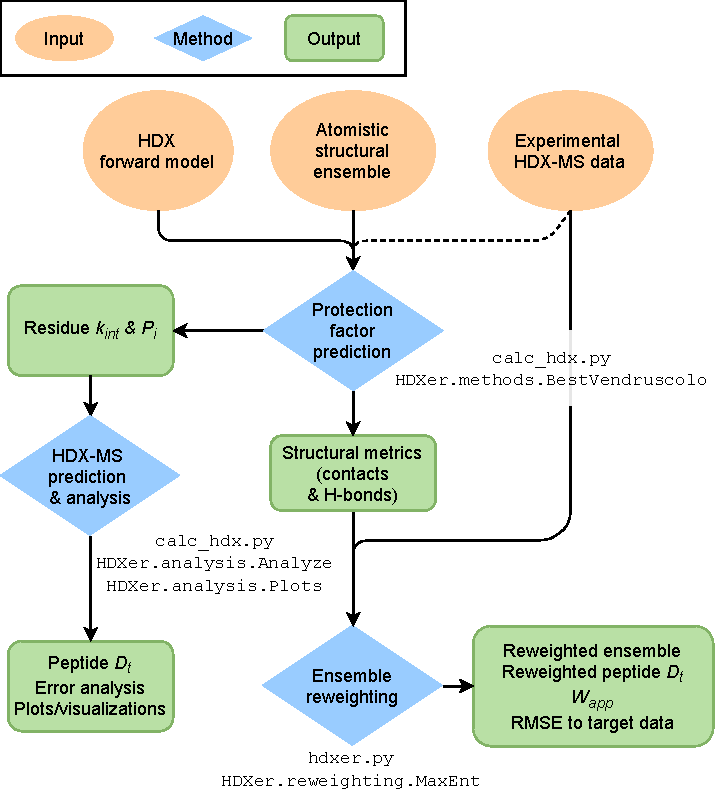
\includegraphics[width=0.98\linewidth]{Fig2_HDXer_workflow_vertical.pdf}
    \caption{Workflow of a typical HDXer analysis. Input structural and experimentally-measured HDX-MS (orange; the dashed line denotes an optional input) can be processed through multiple analysis steps (blue), to obtain predicted HDX-MS data and/or a reweighted structural ensemble as outputs (green). The corresponding software packages or python functions are listed alongside each method. The tutorials cover all aspects of HDXer usage, from preparing input data to interpreting the outputs.}
    \label{fig:workflowfig}
\end{figure}

\subsection{Organization of the tutorials}
The initial stage for any HDXer analysis is the collation and preparation of input data sources, such as the candidate structural ensemble and target (experimental) HDX-MS data, as specified in section \ref{maxent_theory_sect}. 
We describe how to collate such input data in section \ref{collating_inputs}, while tutorial 1 (section \ref{tutorial_1}) provides a practical example of the process, with particular focus on dealing with experimental data from diverse sources.

Having prepared suitable input data, the next stage of an HDXer analysis involves the prediction of protection factors from the candidate structural ensemble, the subsequent calculation of predicted deuteration levels for peptide segments, and comparison with experimental HDX-MS data if desired.
Tutorial 2 (section \ref{tutorial_2}) demonstrates an application of the protection factor and HDX-MS data prediction functionalities.

The final possible HDXer analysis is to reweight the candidate ensemble to fit target (experimental) HDX-MS data.
Tutorial 3 (section \ref{tutorial_3}) describes an example application based on the HDX-MS predictions completed in tutorial 2, and illustrates how to interpret the outputs of reweighting, namely the final structural ensemble, the reweighted HDX-MS data, and the metrics of $W_\textnormal{app}$ and RMSE to the target data. 

% Section 3
\section{Collating inputs for HDXer analyses}\label{collating_inputs}
All inputs to HDXer must be carefully prepared in order to avoid issues ranging from syntax errors to poor structural fidelity, while performing reweighting analyses. 
For this reason, our first tutorial demonstrates how experimental HDX data should be formatted for use as target data for reweighting.
To complement that tutorial, we provide the following guidelines for the curation of input data, which users should follow when designing their own applications.

\subsection{Curating target HDX data}
HDXer assumes that target data was generated with HDX-MS experiments, currently the most widely-used method for measuring deuterium exchange.
Target data must therefore be provided for a set of peptide fragments, at one or more deuterium exposure times. 
For each peptide, HDXer expects absolute fractional deuteration values, i.e., ranging from 0 (undeuterated) to 1 (fully deuterated).
However, many commonly-used HDX-MS analysis software packages (e.g., DynamX [Waters Corporation], HDExaminer [Sierra Analytics], or Deuteros \cite{Lau2021}) report experimental data as the raw difference in peptide mass, $m_t - m_0$, as standard.
Thus, for use with HDXer, these mass differences for each peptide and time point must be converted to fractional deuteration values, by taking into account the peptide length and sequence (i.e., ignoring proline residues), and the back-exchange experienced by the peptide after quenching the deuteration reaction.
The optimal approach for this conversion is to normalize the observed mass differences to those observed in a maximally-labeled control sample, prepared and analyzed at the same time as the experiment samples \cite{Masson2019}.
In the absence of normalization to a maximally-labeled control, calculated deuterated fractions are lower bounds of the true deuteration of each peptide.
The magnitude of back-exchange is typically reported to be \textit{ca.} 30\% of total exchange, but can vary between 10-50\% depending on peptide composition and experimental conditions \cite{Walters2012}.
Thus, excluding a maximally-labeled control normalization could lead to poor agreement between the calculated and experimental deuteration levels and impinge upon the reweighting process.

We note that for users without access to in-house experimental HDX data, it can be challenging to obtain suitable target data from published literature, as the format and information content of reported data have varied greatly.
For example, HDX data obtained from NMR experiments can variously be reported in terms of measured protection factors, exchange rate constants, or absolute exchange rates.
Although all of these data can be converted to deuterated fractions, as required by HDXer, the metadata required to do so (particularly pD, temperature, and buffer composition) may not have been reported.
HDX-MS data from literature sources vary similarly in the amount and style of reported data, and methodological details can also be tricky to uncover.
Prior to including such data in HDXer analyses, users should satisfy themselves of important considerations, including, but not necessarily limited to, the experimental deuteration conditions, the statistical significance of the measured data (see below), and that the chosen peptides exchange under the EX2 kinetic regime only.
Fortunately, for HDX-MS experiments, recent consensus within the community has recognized the importance of standardizing the reporting and deposition of HDX-MS data, which is expected to improve the reliability, accessibility, and utility of such data for computational analyses moving forward \cite{Masson2019}.

A final consideration during target data curation relates to the choice of the most relevant data. 
In theory, the inclusion of all available target data should restrain the potential solutions of the reweighting analysis and improve the spatial resolution and accuracy of the structural interpretations that HDXer can provide.
However, the information content of all experimental datapoints is unlikely to be equal.
Peptides that either remaining fully undeuterated throughout the experimental timecourse, or that reach maximal deuteration immediately at the earliest measurement time, can only provide a lower- or upper-bound to the (average) $P_i$ of the amides within the segment.
A reweighting analysis that targeted undeuterated peptides would therefore be unable to distinguish between alternate highly-protected conformational states.
Likewise, many highly-flexible, deprotected conformational states would be indistinguishable in reweighting analyses targeting fully-deuterated peptides.
Overall, datapoints that do not exhibit significant differences in mass during the experimental timecourse could effectively decrease the signal-to-noise over the entire ensemble, and result in ambiguous structural interpretations.
Therefore, in practice, we recommend that only datapoints for which significant deuteration are reported be included in the target dataset (see e.g. \cite{Hageman2019, Weis2021} for useful methods to determine significance in HDX-MS data).

For data used to compare ensembles obtained for different states, i.e., when reweighting ensembles from experiments carried out under different protein conditions, e.g. apo and holo states, we recommend including only datapoints that show significant mass differences between the two conditions (i.e. significant $\Delta$deuteration).
Again, in practice, if peptides do not exhibit significant $\Delta$HDX between states, it is impossible for a reweighting process to distinguish whether the two states have identical dynamics, whether they have different dynamics with coincidentally identical $P_i$, or whether they have different dynamics and $P_i$ that have been obscured by the magnitude of the experimental uncertainty.
By neglecting peptides with non-significant $\Delta$HDX, only the datapoints that contribute most to the differences between states drive the outcome of the reweighting.

Nevertheless, filtering of the target experimental data may be undesirable if it means key structural regions of interest are removed from the target dataset.
The best approach to data curation may often be to design experimental measurements that are able to characterize the full range of protein dynamics, and that are as sensitive as possible to small differences between states.
Careful optimization of experimental timepoints, temperature, pH, peptide coverage, and redundancy is therefore always recommended as part of the data curation process for HDXer analyses, and for HDX-MS experiments in general \cite{Masson2019}.

\subsection{Curating a structural ensemble}
As mentioned in section \ref{initialensemble_sect}, there are numerous methodologies that can be used to prepare a suitable candidate protein structural ensemble for reweighting.
However, we expect that most HDXer applications will make use of protein structures generated by MD simulations.
HDXer relies upon the MDTraj package to read and analyze biomolecular structures and trajectories, conferring the ability to read coordinate and topology file formats used by most major MD software packages.
For further details users should consult the MDTraj documentation \cite{McGibbon2015MDTraj}.

Although users should plan their MD simulation protocol carefully depending on the specific question at hand, we make the following general recommendations based on our own experience.

First, the sampling obtained using multiple, independent, repeat simulations (using, e.g., different initial seeds) is typically superior to that obtained from a single, long simulation, and allows the convergence of the simulations to be straightforwardly assessed \cite{Hess2002,Faraldo-Gomez2004,Grossfield2019}.
Moreover, sampling from multiple replicates can also be used to interrogate the reproducibility and variance in HDXer analyses.
The reweighting algorithm itself is a deterministic gradient descent procedure.
Thus, the outputs of HDXer analyses will only vary if the inputs (either the target HDX-MS data, the predictive model, or the candidate ensemble of structures) are also varied.
Since, in many cases, users will wish to maintain an identical target dataset and predictive model across all their analyses, the only means by which to assess the uncertainty in the final reweighted ensemble is by varying the input structural ensemble.
In other words, carrying out multiple reweighting experiments with independent candidate ensembles provides a straightforward way to assess the variance in the accuracy of HDX predictions. 
See section \ref{robustness_sect} for more detail.

Second, in common with all MD studies, the length and level of sampling in the simulations should be chosen based on the timescales of the dynamical motions under investigation. 
In general, structural fluctuations over ps to ns timescales may be accessible to conventional, unbiased MD. 
Motions across $\mu$s to ms timescales are likely to require enhanced sampling \cite{Allison2020} (although note that motions only seen on even longer timescales may be associated with global unfolding and EX1-type kinetics, which is as yet unsuitable for HDXer analysis). 
When using enhanced sampling techniques, users should endeavor to include structures that are representative of the equilibrium dynamics within the candidate ensemble, and no others. 
A relevant example is provided by the binding protein TeaA, used during the development of HDXer.
Specifically, bias-exchange metadynamics simulations had been used to sample the complete free-energy landscape of the TeaA conformational changes \cite{Marinelli2011}, but only the unbiased replica of the simulations, which represents the equilibrium dynamics, was used as the prototypical candidate structural ensemble during reweighting \cite{Bradshaw2020}.
An alternative method, for simulation techniques that do not include an unbiased ensemble, would be for users to ensure the initial weights of their frames reproduce a Boltzmann distribution \cite{Torrie1977, Marinelli2021}.
Instructions for assigning initial weights can be found in the HDXer 'docstring' help text.

Third and finally, in an effort to reduce the 'structural noise' present in the candidate ensemble, simulated frames should be statistically uncorrelated from one another.
Of course, the correlation times for protein dynamics are likely to vary between systems.
However, as a rule of thumb we recommend that structures be extracted at no less than 10 ps intervals.

% Section 4
\section{Selecting parameters for HDXer analyses}
HDXer is highly customizable, and almost all the options used during an analysis can be user-specified. 
These parameters can be divided, broadly speaking, into four distinct contributions, namely: (a) intrinsic rates for each amino acid type in different sequence contexts; (b) experimental conditions, such as pD or T, that impact the conversion of deuteration levels to protection factors; (c) other free parameters required by the predictive model; and (d) parameters defining the process of reweighting. 
The values of (a) and (b) are expected to require only minor adjustments for each new application.
The selection of values for (c) and (d) is discussed in the following sections.

\subsection{Parameters for predicting HDX-MS data from structures}\label{choosingbetaparams_sect}
The predictive model (eqn. \ref{pf_model}) used by HDXer to predict protection factors from molecular structures includes two key scaling factors, $\beta_\textnormal{C}$ and $\beta_\textnormal{H}$.
These factors determine the relative contributions of H bonds and contacts to the structural protection attributed to the protein fold, and ultimately define the estimated $\Delta$G of the conformational motions resulting in exchange \cite{VendruscoloPaci2003, BestVendruscolo2006}.
The relative importance of these two structural factors to the energy may vary between, and within, proteins, and so the optimum values of the scaling factors in our empirical predictive model may also vary.
As we introduced in section \ref{predictivemodel_sect}, the default scaling factors used by HDXer ($\beta_\textnormal{C} = 0.35$, $\beta_\textnormal{H} = 2.0$) were originally parameterized using protection factor data for small, globular proteins \cite{BestVendruscolo2006}.
However, for HDX predictions for larger proteins, or those in non-aqueous environments, the default values may not be suitable, and we therefore recommend that users explore the effects of changing $\beta_\textnormal{C}$ and $\beta_\textnormal{H}$ before embarking upon intensive reweighting analyses.

In practice, we propose that users perform such an exploration using a similar approach to that used in the original parameterization.
That is, calculating protection factors using a range of $\beta$ scaling parameters of similar magnitude to those explored by Best and Vendruscolo and assessing the agreement between the predicted and experimental HDX-MS data.
From the resultant parameter surface -- exemplified in figure \ref{fig:contourplot} of tutorial 2 -- users can not only assess the optimal $\beta$ parameters for their system (those that result in the smallest error with respect to the experimental data), but also visualize the sensitivity of the predictive model to small parameter changes.
This process can provide insight into the ideal selection of $\beta$ parameters for a subsequent reweighting analysis, and whether the parameters should be re-optimized as part of that process while the ensemble populations are being shifted.
Moreover, such an assessment can highlight whether the predictive model is at all appropriate for the protein under study, and thereby preempt problems and inaccuracies that might arise during a reweighting study.
We therefore recommend this analysis as a starting point for all HDXer applications.

\subsection{Parameters for ensemble reweighting}
During reweighting itself, there are two additional parameters that merit careful consideration.
The first parameter, known as the \textit{stepfactor}, affects the efficiency and performance of the analysis. 
As detailed in section \ref{maxent_theory_sect}, the process of reweighting iteratively solves a series of equations to determine the relative weights of individual structures in the candidate ensemble.
These final relative weights arise from the $\lambda$ values (see eqn. \ref{Ucorr_eqn}), which are determined by a gradient descent procedure, whose initial step size is controlled by the \textit{stepfactor} parameter.

The choice of \textit{stepfactor} therefore determines the efficiency of the gradient descent procedure.
From a conceptual standpoint, a large value of \textit{stepfactor} will lead to large initial moves in $\lambda$, and consequently more rapid $\lambda$ optimization.
However, as with any other gradient optimization procedure, if the chosen \textit{stepfactor} is too large, users will encounter overshooting, oscillations, or non-convergence of $\lambda$ values.
By contrast, a small \textit{stepfactor} will precisely converge the optimal $\lambda$ values, at the expense of an increased number of iteration cycles (i.e., compute time).
We have provided a small default value of \textit{stepfactor} for the HDXer analyses to err on the side of caution, and to avoid common gradient optimization problems at the expense of computational cost.
However, we recommend that users begin each study with short trials, using a subset of their candidate ensemble, to determine the suitable range of \textit{stepfactor} values for their own applications.
Our tutorials should provide some insight into this process.

The choice of \textit{stepfactor} may also be closely linked to the second key reweighting parameter, $\gamma$.
As described in section \ref{maxent_theory_sect}, modifying $\gamma$ allows the user to control the width of the uncertainty distribution incorporated in the reweighting process (eqn. \ref{KL_eqn}).
Small values of $\gamma$ result in a broad uncertainty distribution, which, in principle, implies low confidence in either the target data, the accuracy of the predictive model, or the structural comprehensiveness of the candidate ensemble \cite{Orioli2020, Hummer2015}.
Accordingly, small values of $\gamma$ result in little bias being applied to the candidate ensemble, and small shifts in population.
\textit{Vice versa}, large $\gamma$ values imply a high degree of confidence in the input data, and hence that the candidate ensemble should be tightly fit to the target data.

In practical applications of HDXer, it is unlikely that users will be able to accurately quantify all the different sources of uncertainty in the input data, and hence identify an 'optimal' $\gamma$ value for their analysis \textit{a priori}.
It is therefore important for users to run multiple HDXer analyses to assess how the apparent work, $W_\textnormal{app}$, and RMSE to the target data, vary across a range of $\gamma$ values \cite{Orioli2020}.
This data can be used for selecting a suitable $\gamma$ value and a corresponding final reweighted ensemble, or conversely to identify overfitting, and is therefore an important part of any statistically robust HDXer analysis.
We provide a practical demonstration of this crucial process in the tutorials described below.

% Section 5
\section{Tutorials}\label{tutorial_sect}

The HDXer tutorials guide the user through each stage of an HDX ensemble reweighting analysis using a series of interactive Jupyter notebooks.
Each Jupyter notebook contains a brief introduction, interactive scripts in Python or Bash, and discussion of the steps involved in reweighting.

The tutorial folders also include the two example data sets required to perform HDX ensemble reweighting: experimental HDX data and a candidate structural ensemble.
Specifically, data for Bovine Pancreatic Trypsin Inhibitor (BPTI) is provided.
BPTI is a small and compact globular protein and has been studied extensively, including using HDX methodologies. 
We complement these experimental HDX data with MD simulation trajectories.

In the tutorials, we walk the user through the following steps:
\begin{enumerate}
  \item Installing the HDXer software
  \item Preparing the experimental HDX data
  \item Predicting HDX levels for an ensemble of BPTI structures
  \item Reweighting the ensemble of BPTI structures to fit the experimental data.
\end{enumerate}

% Section 5.1
\subsection{Installing the HDXer software}
The HDXer software itself is a Python 3.7 package, which the tutorials will assume has been installed and is accessible to the user's Python environment.
Installation of the HDXer package, as described in section \ref{Software_sect}, provides the user with access not only to the scripts that perform HDX ensemble reweighting, but also to the data files and Jupyter notebooks necessary for the tutorials.
Detailed installation instructions can be found on the main page of the HDXer GitHub repository (\url{https://github.com/TMB-CSB/HDXer}); software requirements for the installation are provided in Section \ref{Software_sect}. 

During the installation, the user creates a Conda virtual Python environment specific for HDXer called \texttt{HDXER\_ENV}, which helps to ensure that the necessary dependencies have been installed and that HDX ensemble reweighting produces the expected results. 
The user also creates an environment variable specifying the location of HDXer, \texttt{\$HDXER\_PATH}, allowing easy access to the HDXer directory and simplifying the process of running the scripts.
Although the tutorials are written for use with a Conda virtual environment and Bash shell, the notebooks should be transferable to other environment managers and shells, if necessary, with only minor syntactic modifications, provided that the above naming convention is followed. 
In all cases, we recommend that the user runs the functional tests provided with HDXer to check for a successful installation prior to running the tutorials; instructions can be found in the installation notes provided in the \texttt{README.md} file. 

By now, the user should have the HDXer software installed and access to the materials needed for the tutorials. We encourage the user to follow along with the Jupyter notebooks in the next few sections for an interactive learning experience.
The notebooks can be found in the \texttt{\$HDXER\_PATH/tutorials/notebooks/} folder.

% Section 5.2
\subsection{Tutorial 1: Preparing experimental HDX data for use with HDXer}\label{tutorial_1}

\subsubsection{Introduction}
The first tutorial notebook focuses on ensuring that the data to be used in HDXer is formatted correctly. 
We anticipate that most HDXer users will obtain their data from HDX-MS measurements, so HDXer expects target experimental data to be provided in an HDX-MS style, i.e., fractional deuteration values (also known as relative fractional uptake RFU), for peptide segments, at specific experimental deuterium labeling times. 
However, there are a number of other, interconvertible, metrics that can be used to describe the deuterium uptake of a protein over time. 
For example, NMR data may be quoted in terms of residue-level $P_i$, or $\Delta{G_{exch}}$. 
Therefore, it is important to know how data types can be interconverted. 
In the first step of the tutorial, we will illustrate how to convert residue-level protection factors from NMR experiments into a HDX-MS style dataset suitable for use with HDXer. 
Example scripts can be found in the first Jupyter notebook: \texttt{01\_data\_prep.ipynb}.

\subsubsection{Prerequisites}
For this tutorial, users should be familiar with the general concepts and terminology of mass spectrometry (MS) measurements. 
A familiarity with software used to process HDX-MS experiments will also be useful for users preparing their own data for HDXer analyses.
In particular, knowledge of the contents of processed HDX-MS data files, which are usually in comma-separated value (csv) format, will be necessary to convert files into the space-delimited text format expected by HDXer.

\subsubsection{Tutorial steps and results}

\textit{Gathering required data} -- The experimental HDX data that we will use for BPTI were first reported as observed H-D exchange rate constants for discrete backbone amides, measured by NMR \cite{Kim1993, Battiste2002}. 
However, rate constants for individual residues were measured in different experiments, at various different temperatures and pD values.
As such, the residue-level exchange data cannot be combined into a single data set without first standardizing the exchange rates to a single set of experimental conditions.
In practice, the observed exchange rate constants should be converted into protection factors for each residue, $P_i$, using Equations \ref{pf_model} and \ref{Df_eqn} as described in Section \ref{predictivemodel_sect}.
This is because, conceptually, $P_i$ is a thermodynamic metric independent of the exact experimental conditions used to measure HDX, assuming that the experimental conditions do not modify the structure and dynamics of the protein from the native ensemble.
Conveniently, the original NMR exchange data for BPTI have already been converted to protection factors in a study by Persson \& Halle \cite{Persson2015}.
In this tutorial we will further convert the experimental protection factors into fractional deuteration values for each residue, as if the data had been recorded \textit{via} HDX-MS experiments, rather than NMR. 

The original data, \texttt{BPTI\_expt\_PFs.dat}, are provided in the \texttt{BPTI\_expt\_data} directory.
This file contains protection factors for the majority of, but not all, individual backbone amides in BPTI.
According to Equation \ref{Df_eqn}, conversion of these values to deuterated fractions requires: (\textit{i}) the deuterium labeling times at which to calculate the HDX levels (\textit{t}), and (\textit{ii}) intrinsic rates of exchange ($k_\textnormal{int}$).
Generally speaking, for real HDX-MS target data the timepoints will correspond to the labeling times used during the experiment.
In this tutorial, we will calculate the fractional deuteration at a range of labeling times typical of those covered by bottom-up HDX-MS, namely 0.167, 1.0, 10.0, and 120.0 minutes. 

The second requirement, the intrinsic rate constant for each backbone amide in a protein, depends upon the chemistry of the neighboring residues as well as the temperature and pD of the reaction solution, and can be readily computed from a table of intrinsic rates for each amino acid type.
For the users' convenience, we provide the intrinsic rate constants of each residue in BPTI, computed at pD 7.4 and 298 K, in the file \texttt{BPTI\_Intrinsic\_rates.dat}, which can also be found in the \texttt{BPTI\_expt\_data} directory.
These intrinsic rate constants are based on reference measurements of amide exchange rates in solution, with sequence-based corrections to the rate constants \cite{Bai1993, Nguyen2018}.
These values can also be obtained at a specified pD and temperature using the \texttt{calc\_hdx.py} Python script, as explained in section \ref{calc_hdx_py_sect} below.

With these data in hand, the first steps of the tutorial guide the user through the process of reading in the experimental $P_i$ and $k_{int}$ values.
Although \texttt{BPTI\_Intrinsic\_rates.dat} contains intrinsic exchange rate constants for every non-proline backbone amide in BPTI, note that, as is common, the experimental HDX protection factor data for BPTI does not cover every residue in the protein. 
Therefore, to prepare for the calculation of residue deuterated fractions, the tutorial notebook next compares and filters the arrays of the experimental protection factors and the intrinsic rate constants, to remove residues that are not present in both data sets.

\noindent
\textit{Converting to deuterated fractions} -- Having gathered files containing the protection factors, intrinsic rates, and timepoints, the user is now guided through the steps to compute residue-based HDX deuterated fractions, according to Equation \ref{Df_eqn}.
However, since HDXer expects deuterated fraction data to be provided for peptide segments rather than individual residues, a further formatting step is required.
Specifically, the experimental data text file should space-delimited, with columns detailing (\textit{1}) the starting residue of the current peptide segment, (\textit{2}) the ending residue of the current peptide segment, and (\textit{3 -> n}) the fractional deuteration at each experimental timepoint.
The penultimate step of this notebook provides example Python commands to create such a peptide-level datafile, called \texttt{BPTI\_expt\_dfracs.dat}.

Note that, by default, the first residue in every peptide segment is ignored by HDXer and does not contribute to the average HDX deuterated fraction of each peptide at each experimental timepoint.
This is because HDXer assumes that any deuterium labeling of the first residue in each HDX-MS peptide segment is completely back-exchanged to hydrogen after the quenching of labeling and digestion of the intact protein, as the hydrolyzed amide becomes a new, extremely labile, N-terminal amine.
Accordingly, for residue numbers in the first two columns of the experimental datafile of $a$ and $b$ respectively, corresponding to the first and final residue of a given peptide segment, the calculation will consider only the residues from $a+1$ to $b$.
Thus, in the case of BPTI, the fractional deuteration for HDX-MS peptide segments of length 2 (residue $i-1$ to residue $i$) actually represents the fractional deuteration of individual residue $i$.
This detail should be kept in mind when users prepare their own datasets for use with HDXer.

Finally, by way of visualization, the tutorial invites users to plot the original protection factor values and corresponding deuterium uptake values over time for each residue in the BPTI dataset.
This plot can provide an important 'sanity check' of the correctness of the conversion between HDX experimental data formats, and can also help users to understand the practical relationship between the magnitude of $P_i$ and of $D_{i,t}$ for their protein and experimental conditions of interest (i.e., pD, T, etc.).

\subsubsection{Conclusion}
After completing the first notebook, users should have a clearer understanding of the type of data needed by HDXer, as well as the specifics of processing raw data files into the required formats. 
The next stage involves predicting HDX data from the structural ensemble that is to be reweighted.

% Section 5.3
\subsection{Tutorial 2: Predicting HDX data}\label{tutorial_2}

\subsubsection{Introduction}
The goal of predicting deuterium exchange from structure is to allow direct comparison of predicted and experimental HDX data, and thereby interpretation of the observed HDX in molecular detail.
In the second Jupyter notebook, \texttt{02\_calc\_hdx.ipynb}, we provide details of the predictive model used by HDXer to estimate protection factors and predict HDX-MS data, and guide users through an example HDX-MS prediction using an ensemble of structures of BPTI.
The computational predictions will then be compared with the experimental BPTI data that were prepared during Tutorial 1.

\subsubsection{Prerequisites}
The key requirement for this tutorial is an ensemble of atomistic protein structures, which will be used both for predicting HDX levels and for the later reweighting steps. 
For BPTI, we provide in-house MD simulation trajectories in a repository on Zenodo (\url{doi:10.5281/zenodo.4640760}). 
This repository contains five replica trajectories, each 500 ns long, from five separate simulations of BPTI in solution.
To follow along with all the steps in this tutorial notebook, users should download the entire directory containing all five runs (i.e., \texttt{BPTI\_simulations}), from Zenodo, into the existing \texttt{\$HDXER\_PATH/tutorials/BPTI/} folder.
However, for users short on time or storage space, we also provide a reference set of predicted HDX-MS data, which can be used to follow the visualization and analysis steps of the tutorial. 
These data are available in the \texttt{\$HDXER\_PATH/tutorials/BPTI/BPTI\_calc\_hdx/} folder.

\subsubsection{Tutorial steps and results}\label{calc_hdx_py_sect}

\noindent
\textit{Predicting HDX data from MD simulations} -- In this tutorial we introduce the \texttt{calc\_hdx.py} Python script (see Figure \ref{fig:workflowfig}), a wrapper script that allows users to predict HDX-MS data for an ensemble of structures. 
This script is run using a Unix command line interface and allows the input filenames, method, analysis options, and output filenames to be specified using \textit{via} command-line flags.

In the first step of the tutorial we set up and describe the \texttt{calc\_hdx.py} command to predict HDX-MS data from the BPTI MD trajectories.
We encourage users to review the help text provided by \texttt{calc\_hdx.py} (accessible by running \texttt{calc\_hdx.py -h} on the command line), which explains how to provide input data, specify method options, and name outputs, using the command line flags.

Next, we run \texttt{calc\_hdx.py} to predict HDX-MS data from the BPTI MD trajectories, using a default set of prediction options.
Specifically, we utilize the \textit{BestVendruscolo} method flag, a model named after its developers \cite{BestVendruscolo2006}, to predict protection factors.
As we first showed in Equation \ref{pf_model}, this model uses the number of H bonds and heavy atom contacts formed by each amide NH group to calculate the protection factor for each backbone amide.
By default, HDXer evaluates H bonds and contacts in an identical way to the originally-parameterized model: an H bond is counted if there is a protein oxygen atom found within 2.4 Å of the amide H atom, and heavy-atom contacts are computed as the total number of nearby protein non-hydrogen atoms, within a radius of 6.5 Å of the amide N atom.
Contacts from the sequence neighbors of the amide (residues $i-2$ to $i+2$) are excluded from the total.
The first step of the tutorial explains how users can modify these options, e.g., to replace the distance-based H bond calculation with a combined distance and angle cutoff, or to include a bound ligand in the calculation of contacts and H bonds. 

In addition, users can modify the scaling factors, $\beta_\textnormal{C}$ and $\beta_\textnormal{H}$, that quantify the relative contributions of heavy atom contacts and H bonds to the protection factors.
As mentioned in section \ref{choosingbetaparams_sect}, exploring a range of $\beta$ parameters can provide information regarding the accuracy of the \textit{BestVendruscolo} predictive model for a given protein system and associated set of HDX-MS data.
Since an interactive exploration of $\beta_\textnormal{C}$ and $\beta_\textnormal{H}$ parameters is too time consuming for a tutorial, we instead provide the results of such an analysis for the BPTI data used in the tutorial in Figure \ref{fig:contourplot}.
This analysis demonstrates that, for our BPTI trajectories at least, the optimal values of $\beta_\textnormal{C}$ and $\beta_\textnormal{H}$ are close to their default, originally-parameterized, values of $\beta_\textnormal{C} = 0.35$, $\beta_\textnormal{H} = 2.0$.
We will return to this analysis in Tutorial 3, when deciding whether to automatically optimize $beta$ parameters during the reweighting of the BPTI ensemble.

\begin{figure}
    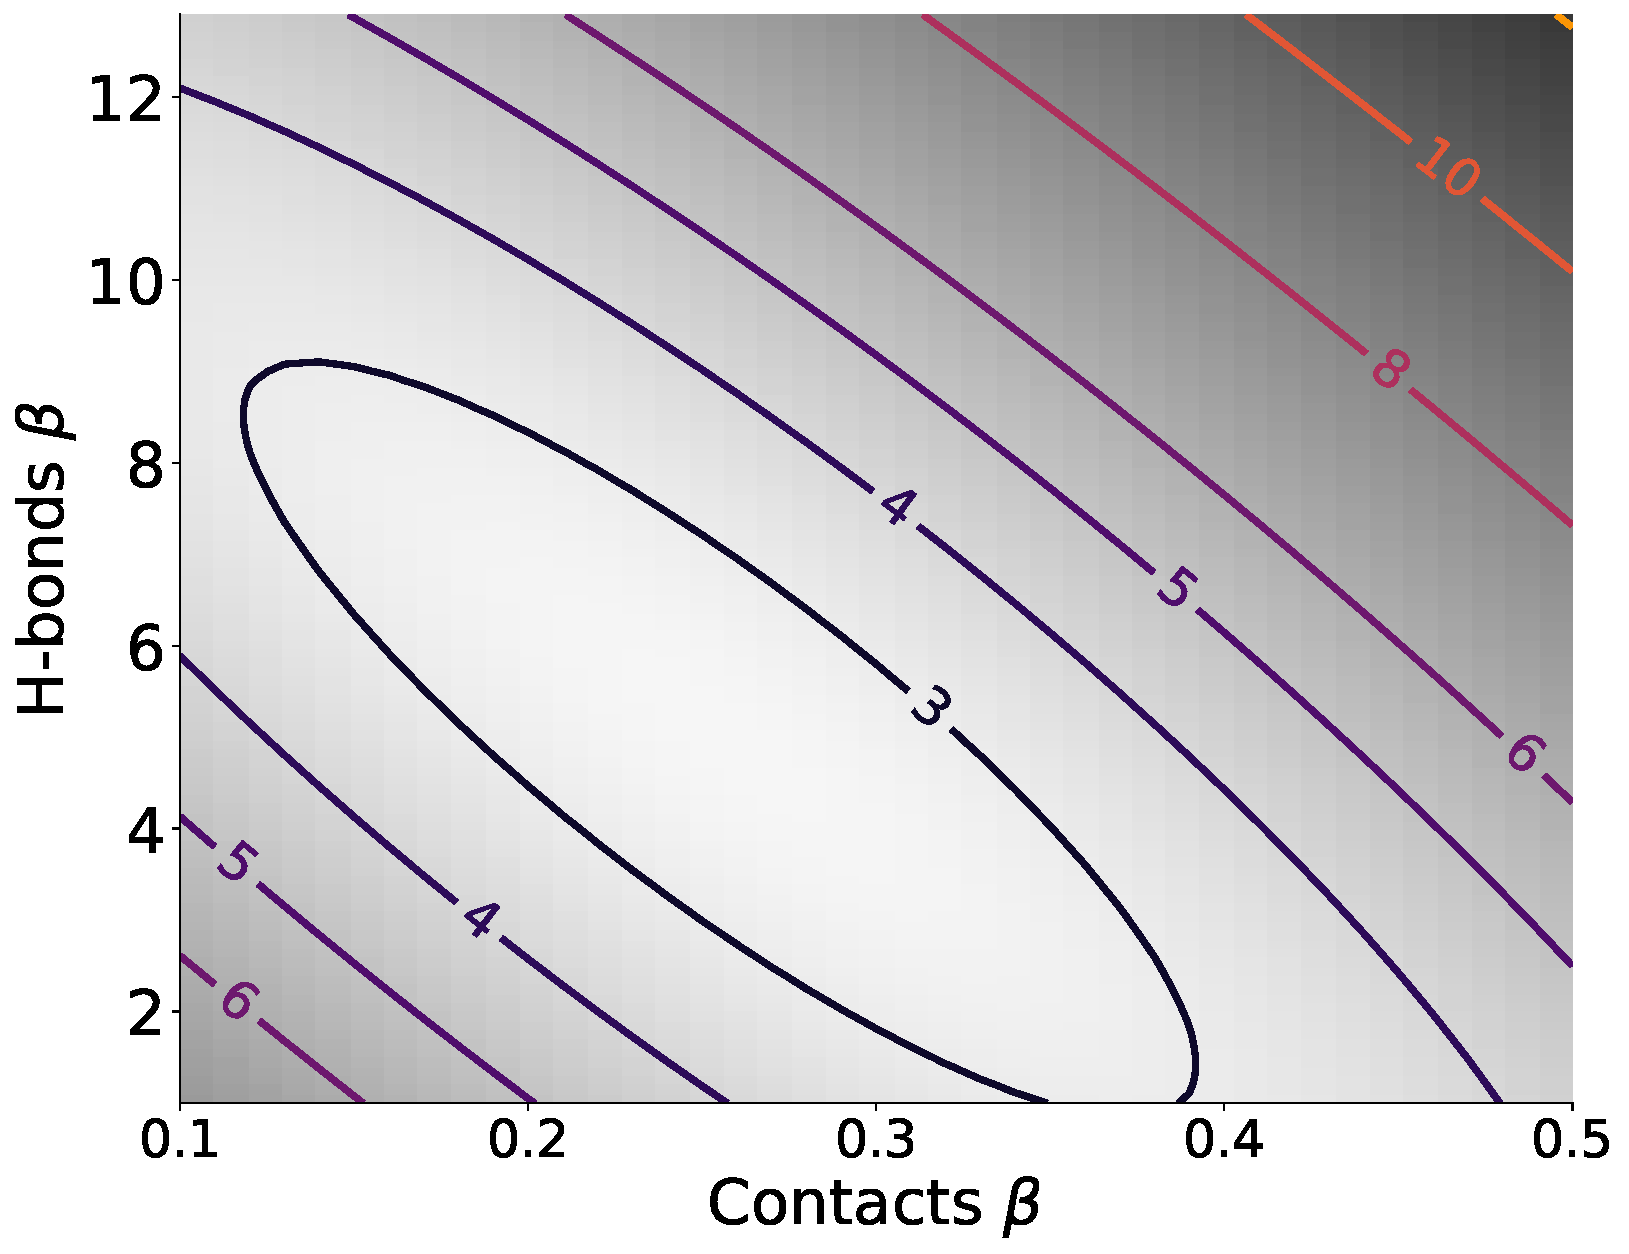
\includegraphics[width=0.98\linewidth]{Fig3_BPTI_noreweight_contour_plot_v2.pdf}
    \caption{Effect of changing the $\beta_\textnormal{C}$ and $\beta_\textnormal{H}$ parameters used to predict HDX-MS data for the BPTI trajectories used in Tutorial 2. Contours indicate the root mean square error in $\textnormal{ln}{P_i}$ as $\beta_\textnormal{C}$ (x-axis) or $\beta_\textnormal{H}$ (y-axis) are varied from their default values, $\beta_\textnormal{C} = 0.35$, $\beta_\textnormal{H} = 2.0$}
    \label{fig:contourplot}
\end{figure}

The final series of \texttt{calc\_hdx.py} options that users are invited to select during the tutorial, relates to the intrinsic exchange rates for each backbone amide.
Intrinsic exchange rate constants, $k_{int}$, will be computed by HDXer automatically, based upon the amino acid sequence of the protein provided to \texttt{calc\_hdx.py} and the temperature and pD conditions at which the experimental data was measured. 
By default, \texttt{calc\_hdx.py} calculates such rates assuming the experiment was performed at 298 K and pD 7.4, but the latter values can be straightforwardly altered \textit{via} the command-line flags, as illustrated in the tutorial.
Finally, to complete the calculation of exchange rates as per equation \ref{Df_eqn}, the user should provide a list of labeling times that reflect the protocol used to generate the experimental data, or else default values will be used.

\noindent
\textit{Plotting predicted HDX data} -- The agreement between the newly-predicted HDX data and the experimental data can be assessed using plots of the deuterated fraction for each peptide fragment.
The tutorial therefore guides users through the creation of such plots, as well as the calculation of some simple descriptive statistics to characterize the agreement between predicted and experimental data. 
The output for BPTI illustrates good agreement for most peptides in the dataset, with an overall $R^2$ for the predictions of 0.59, and a RMSE between the predicted and experimental fractional deuteration values of 0.30. 

\subsubsection{Conclusion}

During Tutorial 2 we predicted HDX data from an ensemble of structures of BPTI and compared the results to experimental HDX data. 
In the case of BPTI, the predicted and experimental HDX data correlate reasonably well ($R^2$ = 0.59), which is not uncommon, but offers clear scope for improvement.
In cases when the correlation is poor, even for only a few individual residues, it can be challenging to distinguish between the multiple possible sources of mismatch, which include errors in the experimental data or the HDX prediction model as well as limitations of sampling in MD simulations. 
Another possibility is that the structural ensemble contains the correct structures, but that they are not in the correct proportion. 
By allowing for reweighting of the structural ensemble, HDXer can robustly account for all these sources of error. 
The next section of the tutorial will describe how to perform reweighting on the BPTI data set. 

% Section 5.4
\subsection{Tutorial 3: Ensemble reweighting}\label{tutorial_3}

\subsubsection{Introduction}

Having completed the first two tutorials, the user should now have all the necessary files to perform reweighting of a candidate ensemble of BPTI structures so that they conform to a target set of BPTI experimental HDX data.
As mentioned above, the process of reweighting applies a minimal bias to the candidate ensemble to identify a structural ensemble that conforms to the experimental HDX data within a given level of uncertainty (equation \ref{KL_eqn}).
The level of uncertainty, and correspondingly the magnitude of bias applied, is controlled by the parameter $\gamma$, which must be chosen by the user and supplied to HDXer for each reweighting analysis.
In practice, to avoid overfitting, reweighting should be carried out in multiple iterations in which $\gamma$ values are varied, and the accuracy of the reweighted data (e.g. the RMSE between the predicted and target HDX) and the bias applied (in terms of $W_\textnormal{app}$) should be evaluated for each iteration.
Tutorial 3 comprises three Juypter notebooks that show the user how to design and carry out an example reweighting experiment (\texttt{03\_reweighting.ipynb}), how to determine a 'suitable' $\gamma$ value in a \textit{post hoc} fashion (\texttt{04\_decision\_plot.ipynb}), and how to analyze the results (\texttt{05\_heatmap.ipynb}). 

\subsubsection{Prerequisites}

Files containing the target experimental HDX-MS data, the intrinsic rates for each protein residue present in the candidate structures, and the residue-level contacts and H bonds used for the HDX predictions, are all required for HDX ensemble reweighting calculations.
Furthermore, the deuterium labeling timepoints associated with the target experimental data are also necessary, although they are provided as keyword arguments to HDXer in a Python script, rather than in a separate file.
Thus, the user should have completed the previous sections of the HDXer tutorials to ensure they are aware of the contents of these files and how they will be utilized within the HDX ensemble reweighting process.

\subsubsection{Tutorial steps and results}

\noindent
\textit{Reweighting with varying levels of allowed uncertainty} -- Within the HDXer package, maximum entropy reweighting analyses are contained within the \texttt{HDXer.reweighting} module.
As such, users can straightforwardly customize and carry out reweighting by writing only a few lines of Python code.
Notebook \texttt{03\_reweighting.ipynb} provides an example of commands to, first, set up a reweighting analysis as a \texttt{HDXer.reweighting.MaxEnt} object, and subsequently to run reweighting interactively across a range of $\gamma$ values, from $\gamma = 1\times10^{-3}$ to $\gamma = 9\times10^{-3}$.

The value of $\gamma$ ultimately determines the level of uncertainty allowed in the fit of the predicted HDX data to the target experimental data. 
That is, higher values of $\gamma$ will cause a larger bias to be applied to the candidate ensemble, resulting in the reweighted data being fitted more tightly to the target experimental HDX data. 
Consequently, the discrepancy, or error, between the final predicted HDX data from the reweighted ensemble and the target experimental HDX data will be reduced.

After performing ensemble reweighting, HDXer produces output files containing the following data: the individual weights (i.e., relative probabilities) of each structure in the ensemble; the final predicted deuterated fractions for that reweighted ensemble; the mean squared error between the predicted and target experimental HDX data; and finally, the 'apparent work' that was applied as a bias to the ensemble as a whole.

By inspecting the output files generated by notebook \texttt{03\_reweighting.ipynb}, users will find that very little bias was applied to the candidate ensemble for the range of $\gamma$ values explored, and therefore the reweighting did not substantially improve the agreement of the predicted and experimental data.
This is deliberate: for the tutorial, these $\gamma$ values were selected so that the iterative reweighting process will converge relatively quickly. 
Specifically, these steps of the notebook should take approximately 10-15 minutes to run on a modern desktop or laptop.
Users can, of course, modify the notebook so that a much wider range of $\gamma$ values are tested, including larger values that will apply higher levels of bias to the underlying BPTI ensemble.
However, to save the user the additional computer time we also provide output files for reweighting analyses performed with $\gamma$ values that range from $1\times10^{-3}$ all the way to $9\times10^{0}$. 
These files will be used in the following notebook, \texttt{04\_decision\_plot.ipynb}.

\noindent
\textit{Creating a decision plot} -- Having performed reweighting with a wide range of $\gamma$ values, to generate a series of reweighted ensembles, the next step is to select an appropriate $\gamma$ value for which the user can inspect the structural effects of reweighting in detail.
However, if the chosen $\gamma$ value is too high, overfitting can readily occur. 

In this context, overfitting means that the final reweighted ensemble has been fitted more closely to the target data than is justified by the uncertainty in the reweighting analysis.
Uncertainty in the analysis can stem from either experimental, predictive model, or structural sampling inaccuracies.
An overfitted ensemble is therefore unlikely to accurately represent the structures present in the experimental HDX-MS sample.
In practical terms, overfitting during reweighting will result in a large increase in applied bias (apparent work), for little improvement in accuracy to the target data.
To identify these situations, we suggest that users create a 'decision plot', also know as an 'L-curve', and apply a heuristic to select an optimal $\gamma$ from the range of tested values.

In notebook \texttt{04\_decision\_plot.ipynb} we therefore create a decision plot of $W_{app}$ \textit{versus} the mean squared error between the predicted and experimental HDX data (Figure \ref{fig:decision_plot}).
The most suitable $\gamma$ for the subsequent analyses, i.e., that producing the closest agreement to experiment without inducing overfitting, can be identified by looking for a sharp elbow, 'L', shape in the decision plot.
In some cases, the potential for multiple sources of uncertainty in reweighting analyses means that overfitting can be a gradual process, and no sharp increase in $W_{app}$ is visible in a decision plot.
In this case, users can apply a cutoff metric to the $W_{app}$ value to keep the applied bias within a reasonable range (e.g., 2-3 $k_BT$). 

\begin{figure}
    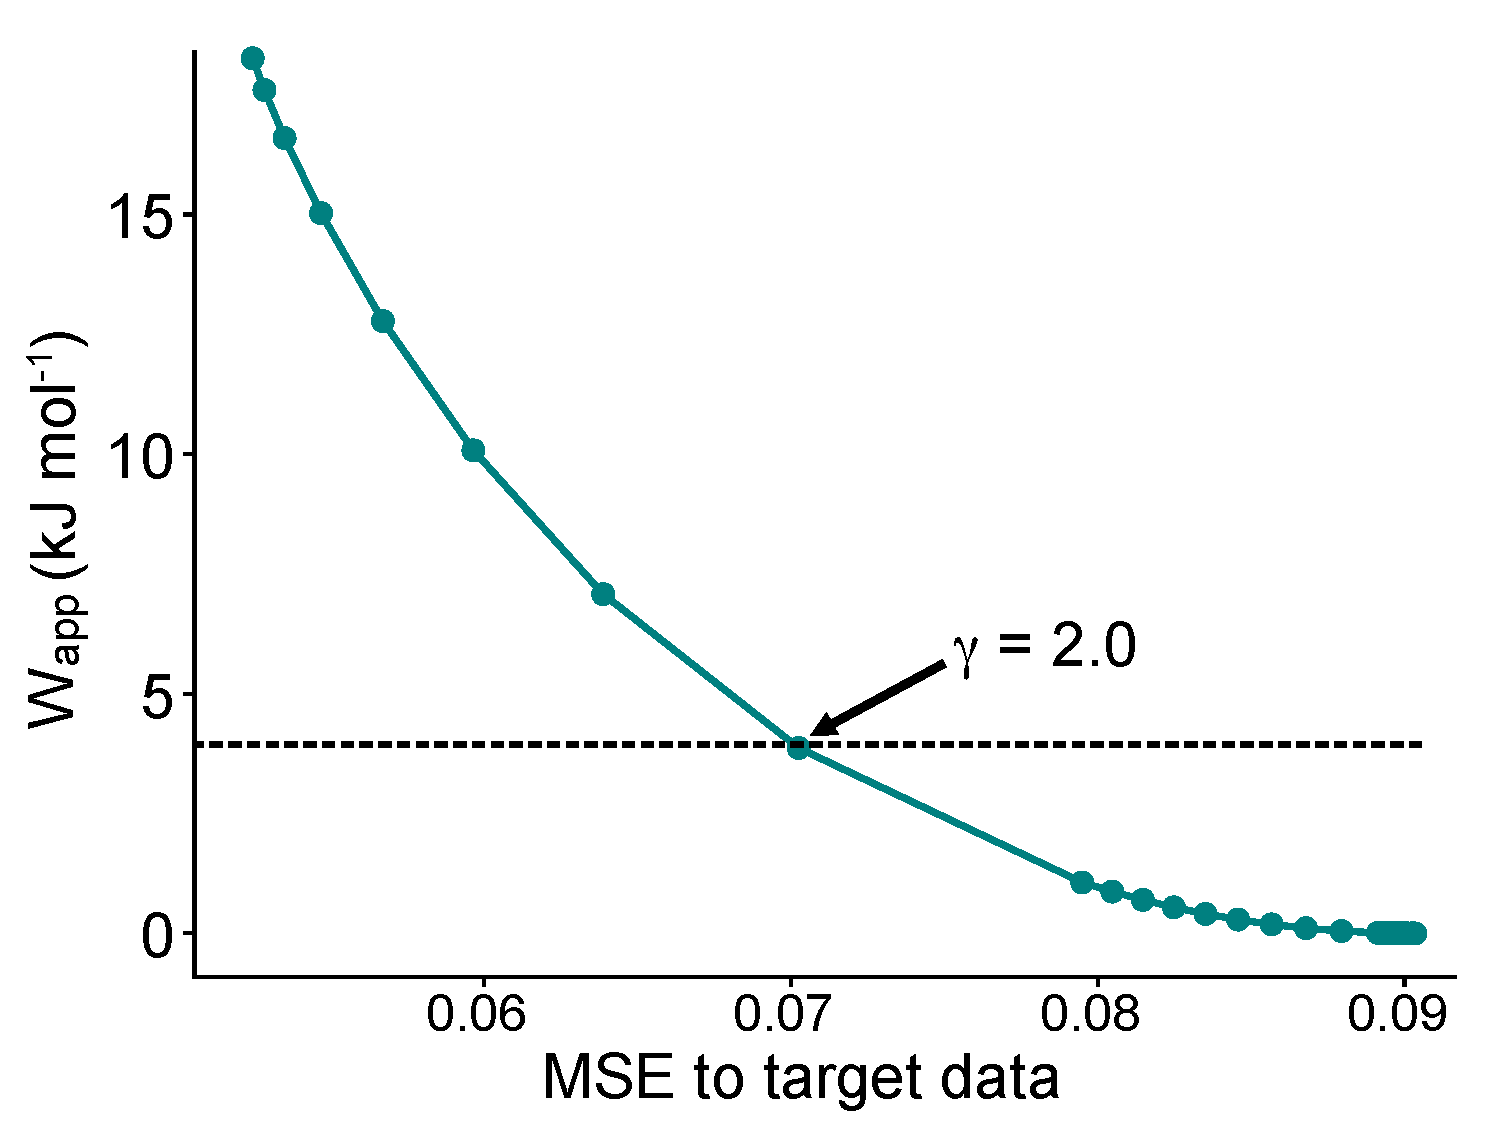
\includegraphics[width=0.98\linewidth]{Fig4_BPTI_decision_plot_LFv2.pdf}
    \caption{Decision plot for the BPTI MD simulation trajectories. An L-shaped curve reveals a sharp increase in work versus the mean squared error, suggesting potential overfitting at values of $\gamma$ leading to higher work values than that at the inflection point. Here, a $\gamma$ value of 2.0 is selected based on the shape of the curve and a cutoff of 4.0 kJ mol$^{-1}$ in the apparent work value (dashed line). The weights obtained at this value of $\gamma$ will be used for further structural interpretation.}
    \label{fig:decision_plot}
\end{figure}

Here, we keep the work value below 4 kJ mol$^{-1}$ (roughly 1 kcal mol$^{-1}$), and choose a $\gamma$ value of $2\times10^0$, based on Figure \ref{fig:decision_plot}.
To visualize the effects of the bias applied at this $\gamma$ value, we plot an overlay of the predicted deuteration values before and after reweighting, which demonstrates how the accuracy of the predicted data (compared to the experimental HDX) improves as a result of reweighting.
An example is shown for the 1-minute labeling time in Fig. \ref{fig:lineplot}.
Finally, we recognize that the choice of $\gamma$ at which to evaluate reweighting is a nuanced decision, and may not always be as straightforward a choice as for the reweighting of BPTI presented in the tutorial.
Interested users can find more discussion of the concepts and practicalities of overfitting, including tests of the sensitivity of ensemble reweighting to the effects of randomly-added noise, in our original article on HDXer \cite{Bradshaw2020}.

\noindent
\textit{Plotting a heatmap} -- After performing reweighting, at the end of notebook \texttt{04\_decision\_plot.ipynb}, users create line plots comparing the predicted values with the target experimental data at each labeling time (see Fig. \ref{fig:lineplot}), providing a simple visualization of how reweighting has improved the agreement of the predicted HDX-MS data with the target data.
However, such visualizations do not readily allow comparison of data from multiple time-points and multiple conditions simultaneously \cite{Masson2019}, and neglect the structural context of the HDX-MS predictions, and thereby the impact of reweighting on the structural ensemble itself.
Therefore, in notebook \texttt{05\_heatmap.ipynb}, we explore some alternative (albeit not exhaustive) ways to visualize the effects of reweighting.

\begin{figure*}[ht]
    \centering
    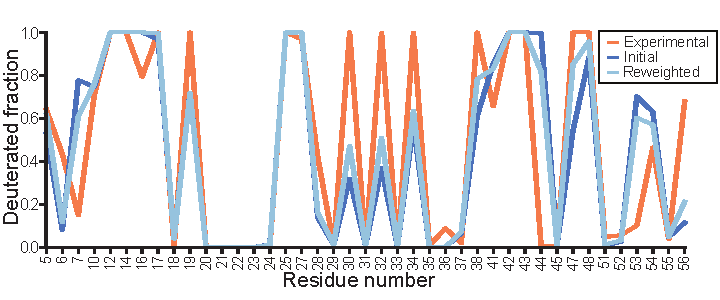
\includegraphics[width=0.9\linewidth]{Fig5_BPTI_lineplot_1min_v3.pdf}
    \caption{Target fractional deuteration values for selected residues in BPTI after 1 minute labeling (orange) overlaid with predicted values obtained before reweighting (dark blue) and after reweighting (light blue). Although H-D exchange is predicted accurately for many residues, some discrepancies between prediction and experiment remain, even following reweighting.}
    \label{fig:lineplot}
\end{figure*}

First, users create a heat map to represent the changes in deuterated fractions after reweighting for each residue and each timepoint simultaneously (Figure \ref{fig:heatmap}A).
In this case, the columns correspond to residues in BPTI for which HDX-MS data was predicted, while the rows represent the time points at which exchange was predicted.
Each pixel is then colored by the $\Delta{D_{i,t}} = D_{i,t,\textnormal{final}} - D_{i,t,\textnormal{initial}}$, meaning that regions colored red exhibit higher levels of deuteration as a result of reweighting, while regions colored blue are predicted to have lower levels of deuteration.

Next, users can interpret the effects of reweighting in a structural context by mapping the same data onto an example BPTI structure (Figure \ref{fig:heatmap}B).
Here, we use a crystal structure of BPTI, but users could equally overlay the $\Delta$D data onto conformations from the candidate BPTI ensemble itself.

At this point, users may wish to probe the structural effects of reweighting in more depth, with additional, independent, analyses of the reweighted structures present in the final ensemble. 
For example, in this case, the impact of reweighting on the final predicted deuterated fractions, represented by the difference between the predicted deuteration before and after reweighting ($\Delta$D), is relatively small across the different labeling times, but is not uniformly distributed across the entire protein. 
In particular, reweighting does not seem to affect the predicted deuteration for residues 19 to 35, some of which showed large discrepancies to the experimental target data initially (Fig. \ref{fig:lineplot}). 
The residual error between the predicted and experimental data in these regions may arise from a variety of sources, and we will discuss possible approaches to delineate the cause of these discrepancies below, in section \ref{robustness_sect}.
Nevertheless, for other regions of BPTI, the final predicted HDX-MS values are in good agreement with the target data, illustrated by closely matching deuteration levels in Fig. \ref{fig:lineplot}, which suggests that the reweighting approach has led to a reasonable description of the structure and dynamics of these regions in the final reweighted ensemble.

\begin{figure*}[t]
    \centering
    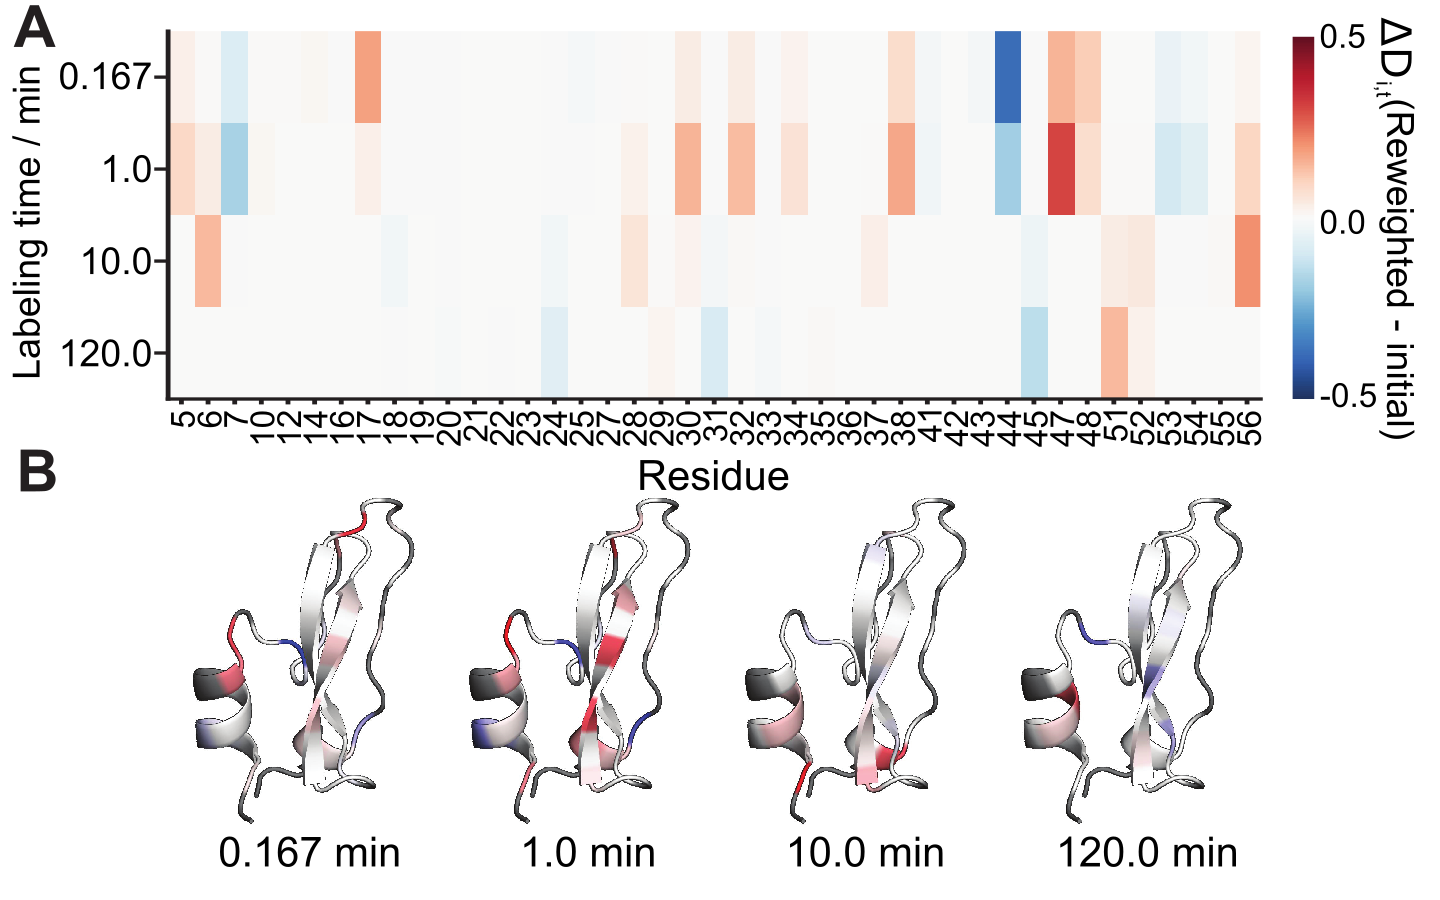
\includegraphics[width=0.9\linewidth]{Fig6_heatmap+structures_2col.png}
    \caption{Effect of reweighting on the predicted deuteration levels in the BPTI structural ensemble. (A) Difference in predicted HDX-MS for each residue at different labeling times shown as a heat map. Red represents an increase in deuteration and blue represents a decrease in deuteration after reweighting. (B) For each labeling timepoint, the difference in HDX is mapped onto an example BPTI crystal structure (protein databank entry 5PTI).}
    \label{fig:heatmap}
\end{figure*}

\subsubsection{Conclusion}

In Tutorial 3, we performed HDX ensemble reweighting for BPTI with simple Python scripts, and tracked the accuracy of the predicted HDX-MS data and the total bias applied to the candidate ensemble across a range of $\gamma$ values.
We discussed how users can choose a suitable $\gamma$ value at which to analyze the final reweighted results, and provided examples of simple analyses and visualizations that users can apply to interpret their data.
Although the examples provided in Tutorial 3 are by no means exhaustive, at this point we expect users will be familiar with the basics of performing HDX ensemble reweighting and analyzing the outcomes, and ready to apply the approach to their own systems and target datasets.
As such, in the final section below, we explain how users can evaluate the reliability and robustness of their own reweighting analyses, in order to confidently understand what information their results can, and cannot, provide.

\section{Minimizing uncertainty and improving robustness}\label{robustness_sect}

A crucial final step for HDXer analyses, to which we have alluded in many sections above, is to ensure that the outputs from reweighting analyses are robust, and that conclusions can be drawn from the reweighted structural ensemble with confidence.
Users will naturally wish to understand how choices made during the HDXer analyses can affect their results, to quantify the uncertainty in their final structural ensemble, and ultimately to validate the accuracy of their conclusions.

An optimal approach to probe the accuracy of HDXer results would be to cross-validate the reweighted structural ensemble against other structural or functional data, and to assess the consistency of the interpretations thereof.
For example, the final reweighted structural ensemble could be used to make predictions of complementary solution-state structural data such as SAXS, SANS, or NMR, or to predict specific structural features such as distance distributions observed in DEER, FRET, or crosslinking-MS experiments.
In making these predictions, users should remember that HDXer applied with the phenomenological predictive model here \cite{BestVendruscolo2006} characterizes predominantly the amide C state structures and dynamics (section \ref{predictivemodel_sect}).
The experimental solution state dynamics will inherently include fluctuations to amide O states, including large or slow transitions not well-captured by HDXer.
For this reason, predictions of alternate experimental data from HDXer ensembles may not be equivalently accurate for all protein systems. 
Nevertheless, for a given protein, cross-validation of the reweighted ensemble may be particularly useful to generate testable hypotheses of the structural effects of mutations or changes in environmental conditions, where we would expect that the relative structural differences between different protein states would be consistently identified by many experimental techniques.

In the absence of external cross-validation there are a number of internal checks that can be performed to validate the self-consistency, and to quantify the uncertainty, of HDXer results.
We discuss some suggested, albeit not exhaustive, checks below.
These checks are designed to probe uncertainties in the final results arising from three potential sources of error: (a) the choice of target HDX-MS data, (b) the choice of the predictive model, and (c) the choice of the candidate ensemble of structures for reweighting.

\subsection{Uncertainty arising from target data}\label{target_data_uncertainty_sect}
An advantage of using HDX-MS data for computational ensemble reweighting, compared to data from other structural biology approaches, is the ability to straightforwardly subsample the experimental measurements.
Bottom-up HDX-MS experiments are performed by sampling the level of deuterium exchange from continuous labeling in solution, at multiple sequential timepoints and for multiple independent, often overlapping, peptides.
Each of these datapoints, of course, is sampled from the same underlying experimental ensemble, and should independently encode protein dynamical information that HDXer can use to fit the weights associated with each candidate structure.
Nevertheless, the experimental uncertainty associated with each measured datapoint may differ, perhaps thanks to minor changes in labeling or analysis conditions during the experiment, or sample variability that affects the structure/dynamics of particular protein regions differently.
Identifying any protein regions or experimental timepoints that result in inconsistent HDXer structural interpretations can therefore be informative regarding the veracity of the target experimental data.

A standard approach used to test the robustness of many model-fitting analyses is to split target data into independent training and test sets.
For HDXer analyses this process is facilitated by the large number of individual (albeit correlated) timepoints and peptide segments that comprise each HDX-MS dataset.
To assess the level of uncertainty across the experimental data, we recommend that users reapply HDXer analyses with systematic variations to the target HDX-MS dataset, and quantitatively assess the differences in the resulting reweighted structural ensemble. 
For example, a systematic 'leave-one-out' approach with target data timepoints can identify whether individual timepoints lead to specific structural interpretations, or \textit{vice versa} result in uncertain predictions.
A similar approach with datapoints of individual target peptides can narrow down the cause of uncertainty to individual regions of the protein, and invite caution in structural interpretations, or highlight the necessity for additional experimental coverage, in those regions.
In summary, \textit{post-hoc} uncertainty assessments of the HDXer target data will be aided if users perform HDX-MS experiments across as many timepoints as practicable, and with as much peptide redundancy as attainable.
We suggest that users take this into account during the experimental design, where possible.

\subsection{Uncertainty arising from predictive model}
HDXer relies on an empirical predictive model (eqn. \ref{pf_model}) to estimate residue $P_i$ from structural metrics.
As we have discussed, the optimal empirical scaling factors of this model may vary for different classes of proteins, particularly where structural protection is afforded by the surrounding environment, e.g., in lipid bilayers.
Thus, as part of the preparation process for HDXer analyses, users are advised to explore a range of different scaling factors to identify parameters well-suited to their system (section \ref{choosingbetaparams_sect}).
Nevertheless, as precise exchange mechanisms may vary \textit{within} a protein, so too may the accuracy of the predictive model used to estimate $P_i$ \cite{Skinner2012models, Mohammadiarani2018, McAllister2015}.
If users wish to investigate the local suitability of the predictive model parameters, we suggest applying a combination of two techniques: i) systematically excluding protein regions from the analysis, and ii) optimizing the predictive model parameters, across a series of HDXer analyses. 

If the predictive model is not representative of a particular experimental exchange mechanism in the protein, errors in HDX-MS predictions will likely correlate with specific protein regions, rather than being uniformly distributed across the whole range of target data.
To assess the presence of such errors, users can repeat HDXer analyses after excluding target data for all peptides in a particular protein region.
This would include all datapoints that correspond to a particular location according to the sequence or structure, and may include multiple, overlapping, peptide segments.
For each repeated reweighting analysis, users can subsequently optimize the predictive model $\beta_\textnormal{C}$ and $\beta_\textnormal{H}$ parameters for the remaining protein regions, either by gradient optimization, Monte Carlo optimization, or Monte Carlo sampling, which can be selected using corresponding Python arguments to HDXer as exemplified in the tutorial notebooks.
If the optimal $\beta_\textnormal{C}$ and $\beta_\textnormal{H}$ remain consistent as each region of the protein is excluded from the analysis, the predictive model is likely to be equally suited to all protein regions.
By contrast, if the optimal parameters for individual regions vary beyond the range that the user would expect, according to the parameter exploration of section \ref{choosingbetaparams_sect} (e.g. Figure \ref{fig:contourplot}), this might suggest that a single predictive model cannot estimate $P_i$ for some protein regions with equal accuracy.
In that event, and assuming that other sources of error are thought to be consistent across each protein region, users may choose to repeat their HDXer analyses using target data divided into sets, each set encompassing a given protein region, and each associated with a different predictive model.
The structural effects of reweighting should then be analyzed separately for each protein region.

\subsection{Uncertainty resulting from candidate ensemble}\label{ensemble_uncertainty_sect}
The final source of error in HDXer analyses is perhaps the most straightforward for users to identify and characterize.
As we have referenced throughout the tutorials, an ideal candidate ensemble for reweighting should cover all 'experimentally-relevant' protein conformational states but contain very few conformations not present in the experiment.
Extraneous, non-experimental, protein conformations pose a challenge because they must be downweighted in order to amplify the 'signal' of structural motifs that conform well to the experimental HDX-MS data.
This 'structural noise' can arise either from insufficient sampling in the generation of the candidate ensemble, or from systematic sampling of conformations that are not present in the experimental ensemble (for example, if apo conformations are included in an ensemble being reweighted to fit HDX-MS data of a holo protein-ligand complex).
The presence and the quantitative effects of any uncertainty in the candidate structures can be interrogated using a combination of two approaches.

Random uncertainty in the HDXer predictions can be characterized by repeating identical HDXer analyses with smaller random subsamples (\textit{ca.} 10-33\% of the full population) of the candidate ensemble.
By applying this bootstrapping-style approach to the structures in the candidate ensemble, users can estimate the mean and confidence intervals of conformational populations in the final reweighted ensemble.
In the event that users have already generated the candidate ensemble from independent MD simulations, an alternative approach to characterize the variance in sampling would be to simply average the reweighting results from HDXer analyses applied to each simulation separately.
However, from our experience we recommend applying the bootstrapping approach to an ensemble combining all independent simulations together, rather than analyzing each simulation separately, since even subtle differences in the structures sampled by each simulation can lead to systematically different HDXer results.

To test for systematic errors in the candidate structures, users should begin by performing a thorough structural analysis in order to classify and quantify each conformational state present in their initial ensemble.
Then, following a similar approach to that used above to identify systematic errors in the target data, users can perform repeated HDXer analyses using subsections of the candidate ensemble, systematically excluding each classified conformational state from the initial ensemble. 
The contribution of the remaining conformational states can then be quantified with respect to the final $W_{\textnormal{app}}$ value, the RMSE to the target data, and to the resultant reweighted populations, whether up- or down-weighted.
If excluding a particular conformation from the candidate ensemble results in reweighting with either (a) improved (smaller) RMSE to target with an equivalent applied $W_{\textnormal{app}}$, or (b) improved (smaller) $W_{\textnormal{app}}$ required to achieve an equivalent RMSE to the target data, then the excluded conformation is unlikely to be present in the experimental ensemble and can be safely excluded from the interpretation of the target HDX-MS data.
However, if large RMSE to the target data remains, regardless of the selected conformational ensemble and applied $W_{app}$, this might suggest that neither any structural state sampled by the MD simulation, nor any population mixture of sampled states, represents the experimental ensemble well.

\subsection{Considerations in experimental design}
The previous sections provide a number of practical approaches to assess and rectify any ambiguities in the computational reweighting applied by HDXer.
However, any ambiguities that arise from the experimental data itself will be challenging and time-consuming to understand using the \textit{post hoc} HDXer analyses described above.
For example, if the HDX-MS experiments are known to probe a highly diverse conformational ensemble, with many states of varied populations, lengthy testing may be required to validate that the HDXer reweighted ensembles cover the complete experimental ensemble.
Users should therefore carefully consider the design and analysis of their HDX-MS experiments from the outset.
Below, we include some key points for HDX-MS experimental design that arise from our own experience of HDXer analyses.

Many HDX-MS experiments are designed to probe molecular complexes, for example in epitope/paratope mapping, or protein-ligand binding studies.
In this case, it is crucial to consider the thermodynamics and kinetics of the molecular association during the experiment.
Users should carefully choose protein/ligand concentrations, equilibration times, and dilution ratios to ensure that the system studied is both at equilibrium, and as monodisperse as possible, during the experiment.
Otherwise, experimental solutions that contain a mixture of conformational states, or states that interconvert over experimental timescales, may give rise to HDX-MS signals that are particularly challenging to interpret.
To avoid this, HDX-MS can be coupled to additional structural techniques, ranging from size-exclusion chromatography to native MS, for sample quality assurance \cite{Masson2019,OBrien2018}.

Assessing the quality of the obtained MS data is also crucial for reliable HDXer analyses.
First, data should be inspected and carefully filtered to remove as much uncertainty as possible from the measured deuterium uptake values.
For example, selecting peptides based on intensity (i.e. signal/noise ratio), and monitoring for artifacts (e.g. signs of aggregation) in mass envelopes, can minimize uneven redundancy across the protein and maximize the representation of peptides with state-to-state differences.
Second, because predictive protection factor models are only applicable to exchange events with EX2-type behavior, peptides that exhibit EX1 or mixed EX1/EX2 behavior should be excluded.
Furthermore, since peptides can manifest different exchange regimes over the timescale of an HDX-MS experiment, users should consider removing all data from labeling times at which EX1 behavior is observed, in order to minimize the uncertainty present in the remaining (shorter) experimental labeling time data.

The suggestions provided above will aid the selection of reliable HDX-MS data as a target for reweighting analyses, but do not guarantee that every datapoint is uncertainty-free.
Thus, careful experimental design is not a substitute for assessing the robustness of the HDXer reweighted ensembles, using the methods described in sections \ref{target_data_uncertainty_sect}-\ref{ensemble_uncertainty_sect}.
Instead, well-characterized, high-quality experimental data will simplify the quality control steps of HDXer analyses, and enhance the accuracy and reliability of the structural interpretations.
Accordingly, we recommend that both components (i.e., experimental and computational) be considered and designed in tandem.
Such a strategy results a single, integrative, HDX-MS and HDXer workflow, that, in our experience, is most likely to succeed in producing in an unambiguous answer to the biological question of interest.


\section{Author Contributions}
%%%%%%%%%%%%%%%%
% This section must describe the actual contributions of
% author. Since this is an electronic-only journal, there is
% no length limit when you describe the authors' contributions,
% so we recommend describing what they actually did rather than
% simply categorizing them in a small number of
% predefined roles as might be done in other journals.
%
% See the policies ``Policies on Authorship'' section of https://livecoms.github.io
% for more information on deciding on authorship and author order.
%%%%%%%%%%%%%%%%

Conceptualization, all authors; methodology development, software development, data curation, and analysis, PSL, RTB, and FM; software testing, KK, AS, PLW, and DJD; writing of original drafts and visualization of data, PSL, RTB, and LRF; writing - review and editing, all authors; supervision, PLW, DJD, JDFG, and LRF; resource and funding acquisition, JDFG and LRF; project administration, RTB and LRF.

For a more detailed description of author contributions,
see the GitHub issue tracking and changelog at \githubrepository.

\section{Potentially Conflicting Interests}
%%%%%%%
%Declare any potentially competing interests, financial or otherwise
%%%%%%%

The authors declare no potentially conflicting interests.

\section{Funding Information}
%%%%%%%
% Authors should acknowledge funding sources here. Reference specific grants.
%%%%%%%
This research was supported by the Division of Intramural Research of the NIH, National Institute of Neurological Disorders and Stroke (to LRF) and the National Heart, Lung and Blood Institute (to JDFG).

\section*{Author Information}
\makeorcid

\bibliography{hdxer_draft_better}

%%%%%%%%%%%%%%%%%%%%%%%%%%%%%%%%%%%%%%%%%%%%%%%%%%%%%%%%%%%%
%%% APPENDICES
%%%%%%%%%%%%%%%%%%%%%%%%%%%%%%%%%%%%%%%%%%%%%%%%%%%%%%%%%%%%

%\appendix


\end{document}
